\documentclass[10pt]{article}
\usepackage[preprint]{tmlr}

\usepackage{amsmath,amssymb,amsfonts}
\usepackage{booktabs}
\usepackage{array}
\usepackage{multirow}
\usepackage{microtype}
\usepackage{xcolor}
\usepackage{tikz}
\usetikzlibrary{arrows.meta,positioning,fit,backgrounds}
\usepackage{pgfplots}
\pgfplotsset{compat=1.18}
\usepackage{hyperref}

\definecolor{tmlrblue}{RGB}{27,79,138}
\definecolor{tmlrorange}{RGB}{196,90,26}
\definecolor{tmlrteal}{RGB}{24,128,112}
\definecolor{tmlrred}{RGB}{172,42,42}
\definecolor{tmlrgray}{RGB}{95,102,110}

\hypersetup{
    colorlinks=true,
    linkcolor=tmlrblue,
    citecolor=tmlrblue,
    urlcolor=tmlrblue
}

\newcommand{\vect}[1]{\mathbf{#1}}
\newcommand{\pp}{\,\text{pp}}
\emergencystretch=3em
\let\origunderscore\_
\renewcommand{\_}{\origunderscore\allowbreak}

\title{In-Place Span Overwrite vs.\ Append for Editable Compressed Context in Frozen LLMs, with Task-Dependent Diagnostics of Short-Budget Latent Prefixes}

\author{\name Ariel Fikru \email github.com/arielfikru/lslc-research \\
\addr Independent Researcher \quad|\quad DOI: \href{https://doi.org/10.5281/zenodo.24473281}{\texttt{10.5281/zenodo.24473281}}}

\begin{document}
\setlength\aftertitskip{0.2in}
\maketitle
\vspace{-1.6em}

{\renewcommand{\thefootnote}{}\footnotetext{This manuscript (v3) supersedes an earlier preprint under the same Zenodo concept DOI after controlled causal ablations established that verbatim state-edit recovery was carried by the discrete footnote bank rather than the co-trained continuous latent delta.}}

\begin{abstract}
Long-horizon assistants over mutable documents face a trade-off between raw-text retrieval---which preserves surface tokens at the cost of long prompts and stale-history conflicts under append-only errata---and compressed context memory, which shrinks active memory tokens but risks discarding or corrupting updated facts. We conduct a controlled study on two strictly frozen BF16 Transformer backbones (\texttt{Qwen/Qwen3-1.7B} and \texttt{unsloth/\allowbreak Meta-Llama-3.1-8B-Instruct}, $r=0$) comparing (i)~a gated discrete span-bank (\texttt{PathBDiscreteMemory}, denoted \texttt{OW-192}; $326{,}407$ trained parameters on \texttt{Qwen3-1.7B}, $594{,}695$ on \texttt{Llama-3.1-8B-Instruct}, with frozen \texttt{bge-small-en-v1.5} routing) against fixed-budget rolling-tail append (\texttt{App-192}) and schema-aware rule-based raw-text overwrite (\texttt{Raw-OW}), and (ii)~a short-budget co-trained input-space continuous latent prefix (\texttt{LSLC-Full}; $400+250+400 = 1{,}050$ post-adapter steps atop a prior adapter release on \texttt{Qwen3-1.7B}; $120$-step probe on \texttt{Llama-3.1-8B-Instruct}).

Three scoped findings emerge.
\textbf{(1)~Controlled State Revision:} On structured multi-turn revisions (\texttt{Gate-2}, $2\times 4$ factorial, $N=200$/backbone, $192$ active memory tokens excluding prompt/query, shared oracle write addresses $p_i$, $0.0\%$ FAR/FRR gate, and $4$ pages locked by \texttt{OW-192}'s post-edit router), \texttt{OW-192} beats $31$-token rolling-tail \texttt{App-192} by $+15.0\pp$ / $+11.0\pp$ (\texttt{ed\_last}/\texttt{id\_asc}) on \texttt{Qwen3-1.7B} ($p_{\text{Holm}}\le 6.78\times 10^{-4}$; cluster CI $[+4.9\%, +17.8\%]$) and $+9.5\pp$ / $+9.0\pp$ on \texttt{Llama-3.1-8B-Instruct} ($p_{\text{Holm}}\le 3.73\times 10^{-3}$; CI $[+2.3\%, +15.8\%]$; cluster sign-flip $p_{\text{sf,H}}\le 0.015$ Qwen vs.\ $0.126$--$0.130$ single-seed Llama). Two disjoint \texttt{Qwen3-1.7B} seeds ($N=400$) replicate $+15.0\pp$ ($77.8\%$ vs.\ $62.8\%$, $66$--$6$, CI $[+9.3\%, +20.8\%]$). Against schema-aware \texttt{Raw-OW} ($\sim 1{,}030$ memory tokens), \texttt{OW-192} scores $+3.5\pp$ to $+6.0\pp$ higher on \texttt{Qwen3-1.7B} ($p_{\text{Holm}}\ge 0.091$) but is \emph{outperformed} on \texttt{Llama-3.1-8B-Instruct} by $-3.5\pp$ / $-6.5\pp$ Norm-EM (CI $[-13.5\%, -0.9\%]$ \texttt{id\_asc}), $-5.0\pp$ / $-8.5\pp$ W2N-EM ($p_{\text{Holm}}=0.0116$, CI $[-16.0\%, -2.6\%]$), and $90\%$ vs.\ $99\%$ ($78\%$ vs.\ $91\%$ \texttt{id\_asc}) on mutable queries.
\textbf{(2)~Task-Dependent Latent Prefix Diagnostics:} On masked-old verbatim probes ($N=24$), the frozen decoder outputs $0/24$ edited values on both backbones without bank updates (vs.\ $24/24$ with bank updates); $\vect{Z}_{\text{book}}$ worsens \texttt{WikiText-2} PPL ($25.91\rightarrow 39.86$ Qwen3; $14.08\rightarrow 17.89$ Llama-8B) and collapses \texttt{Qwen3-1.7B} coding ($1/24$ vs.\ $20/24$, $p=3.81\times 10^{-6}$), yet \emph{improves} legacy suffix-overwrite \texttt{Gate-2} on \texttt{Qwen3-1.7B} ($383/600$ vs.\ $351/600$, $p=2.56\times 10^{-4}$).
\textbf{(3)~Empirical Boundaries:} On \texttt{LongMemEval} \texttt{knowledge-update} ($N=72$, evaluated strictly in static read-only mode with $0$ edit calls and gold-session packing), $48/256$ pruning trails raw-text RAG on \texttt{Qwen3-1.7B} ($9.7\%$--$15.3\%$ vs.\ $26.4\%$ extracted EM) and scores $23.6\%$--$31.9\%$ vs.\ $31.9\%$--$37.5\%$ on \texttt{Llama-3.1-8B-Instruct} as a lexical-coverage proxy drops from $68\%$--$79\%$ to $25\%$--$39\%$. On $4\text{K}$ static contexts, per-head \texttt{SnapKV-style} eviction remains stronger in PPL and $8\text{B}$ QA at the cost of per-query prefill, and partitioned two-bank KV reuse verifies $0.0$ Bank-1 KV drift on repeat edits but runs at $0.82\times$--$0.95\times$ speed ($5\%$--$22\%$ slower) under eager \texttt{DynamicCache}.
\end{abstract}

% ===========================================================================
\section{Introduction}
\label{sec:intro}
% ===========================================================================

Autoregressive language models deployed as long-horizon assistants must repeatedly retrieve and update external state---project budgets, deployment modes, software interfaces, or evolving user facts---without modifying frozen base weights. Two widely used memory designs expose complementary trade-offs:

\begin{enumerate}
    \item \textbf{Raw-Text Retrieval-Augmented Generation (RAG)}~\citep{lewis2020rag,robertson2009bm25,xiao2024bge} avoids full-context quadratic attention by retrieving top-$k$ chunks per query. However, simple append-only errata policies leave superseded records verbatim inside the prompt, creating contextual knowledge conflicts~\citep{longpre2021conflict} and positional recency sensitivities~\citep{liu2024lost}, whereas in-place chunk rewriting requires either brittle domain-specific rules or autoregressive LLM calls~\citep{packer2023memgpt,chhikara2025mem0}.
    \item \textbf{Compressed Context Memory} shrinks active memory prefixes via \emph{continuous soft-prompt encoders}~\citep{mu2023gist,chevalier2023autocompressors,ge2024icae,cheng2024xrag,li2025compressor500x,fallahpour2026memorilla} or \emph{discrete token pruning and KV eviction}~\citep{pan2024llmlingua2,chirkova2025provence,zhang2023h2o,li2024snapkv}. Most discrete pruners and KV evictors target static read-only prompts, while input-space continuous latent compressors atop frozen LLMs have rarely been tested under \emph{in-place state mutation}, where exact verbatim symbols must supersede stale facts without degrading unrelated syntax or language modeling.
\end{enumerate}

This paper conducts a controlled diagnostic and empirical investigation across two strictly frozen BF16 GQA model families---\texttt{Qwen/Qwen3-1.7B}~\citep{yang2025qwen3} and \texttt{unsloth/Meta-Llama-3.1-8B-Instruct} (an ungated BF16 mirror of Meta's Llama-3.1-8B-Instruct~\citep{dubey2024llama3}, $r=0$)---centered on two scoped questions:

\begin{enumerate}
    \item \textbf{In-Place Span Overwrite vs.\ Append in Mutable Compressed Memory (Section~\ref{sec:gate2}):} Given a lightweight gated discrete span-bank (\texttt{PathBDiscreteMemory}, denoted \texttt{OW-192}; $326\text{K}$--$595\text{K}$ trained parameters, $0$ latent encoder, $0$ $\vect{Z}_{\text{book}}$), how much of structured revision accuracy comes from span-aligned in-place overwrite vs.\ fixed-budget rolling-tail append (\texttt{App-192}), page ordering (\texttt{edited\_last} vs.\ \texttt{page\_id\_asc}), or compression relative to schema-aware raw-text overwrite (\texttt{Raw-OW})? We isolate these factors in a $2\times 4$ locked-page, locked-order factorial design ($N=200$ per backbone) plus multi-seed end-to-end and blind-routing evaluations, and map operational boundaries on \texttt{RULER-style} $4\text{K}$--$32\text{K}$ retrieval, \texttt{SnapKV-style} eviction, $65$-file coding, partitioned two-bank KV reuse (Section~\ref{sec:systems}), and static extractive QA over \texttt{LongMemEval} \texttt{knowledge-update} ($N=72$, Section~\ref{sec:lme}).
    \item \textbf{Task-Dependent Diagnostics of Short-Budget Co-Trained Latent Prefixes (Section~\ref{sec:diag}):} Starting from a Perceiver-style~\citep{jaegle2021perceiver} input-space continuous latent book ($\vect{Z}_{\text{book}}$) updated via gated delta-writes (\texttt{LSLC-Full}) trained at short adapter budgets ($400+250+400 = 1{,}050$ post-adapter steps atop a prior adapter release on \texttt{Qwen3-1.7B}; $120$-step confirmation probe on \texttt{Llama-3.1-8B-Instruct}), when does the continuous latent prefix assist vs.\ fail? Using a $5$-cell iso-token masked-old edit probe, locked-page Python coding, \texttt{WikiText-2} continuation perplexity, and multi-seed state revision, we observe a sharp task-dependent interaction: $0/24$ masked-old verbatim readout on both backbones, coding collapse ($1/24$ vs.\ $20/24$) and higher PPL, yet a positive assist under legacy suffix-overwrite \texttt{Gate-2} ($383/600$ vs.\ $351/600$).
\end{enumerate}

\paragraph{Experimental Scope and Statistical Contract.}
We do \emph{not} claim a general replacement for raw-text RAG, general superiority over raw-text overwrite, or impossibility of heavily pretrained continuous context compression. Throughout the paper: (a)~$192$ denotes \emph{active memory tokens} ($4\text{ pages}\times 48\text{ tokens}$), whereas task instructions, $2$-shot formatting examples, and the query add to total prompt length; (b)~in our controlled \texttt{Gate-2} write-policy comparisons (Section~\ref{sec:gate2_factorial}), all four write policies receive the same oracle edit page address $p_i$ during ingestion (blind edit-page routing is evaluated separately in Section~\ref{sec:gate2_e2e}) and are evaluated conditionally on the $4$ pages selected by \texttt{OW-192}'s post-edit router; (c)~primary \texttt{Gate-2} inference uses exact two-sided McNemar tests computed from unrounded discordance counts with Holm--Bonferroni adjustment across all $m=12$ pre-specified contrasts per metric per backbone ($m=6$ on \texttt{LongMemEval}), paired with nominal $B=2{,}000$ percentile cluster-bootstrap $95\%$ CIs resampling $( \texttt{mode}, \texttt{query\_type}, \texttt{gold} )$ clusters (\texttt{seed=2029} for \texttt{Qwen3-1.7B} factorial, \texttt{seed=2026} for \texttt{Llama-3.1-8B-Instruct} factorial and end-to-end runs) and an exact cluster-level sign-flip sensitivity test.

% ===========================================================================
\section{Related Work}
\label{sec:related}
% ===========================================================================

\paragraph{Continuous Latent Context Compression.}
\textbf{Gist Tokens}~\citep{mu2023gist}, \textbf{AutoCompressors}~\citep{chevalier2023autocompressors}, \textbf{ICAE}~\citep{ge2024icae}, \textbf{xRAG}~\citep{cheng2024xrag}, \textbf{500xCompressor}~\citep{li2025compressor500x}, and \textbf{Memorilla}~\citep{fallahpour2026memorilla} compress text segments into compact continuous embeddings or KV states injected as soft prompts, often using Perceiver-style~\citep{jaegle2021perceiver} cross-attention. These methods target read-only compression and typically rely on large-scale pretraining or full-model adaptation. Our diagnostic experiments probe the complementary regime of short-budget co-trained input-space soft prefixes atop strictly frozen LLMs under verbatim state edits, revealing task-dependent failure on masked verbatim readout and Python coding alongside a modest assist when a legacy discrete bank suffers suffix corruption.

\paragraph{Discrete Prompt Pruning and Extractive Compression.}
\textbf{LLMLingua-2}~\citep{pan2024llmlingua2} frames prompt compression as token classification distilled into an encoder, and \textbf{Provence}~\citep{chirkova2025provence} combines RAG pruning with reranking using $100\text{M}+$ encoders on read-only prompts. Our discrete span-bank uses a $183\text{K}$--$316\text{K}$ \texttt{SalienceGate} over frozen token embeddings to keep three $16$-token spans per page, extends extractive storage to \emph{gated in-place span overwriting}, and quantifies where $18.75\%$ token retention succeeds (template-regular entities and structured code) vs.\ degrades (dense multi-session dialogue in \texttt{LongMemEval}~\citep{wu2025longmemeval}).

\paragraph{KV-Cache Eviction, Serving Prefix Reuse, and Editable KV Memory.}
\textbf{StreamingLLM}~\citep{xiao2024streamingllm} and \textbf{H2O}~\citep{zhang2023h2o} evict KV entries using attention sinks and heavy-hitter scores, whereas \textbf{SnapKV}~\citep{li2024snapkv} pools observation-window attention per head to keep clustered KV spans before generation. Our local \texttt{SnapKV-style} implementation reproduces per-head 1D pooling via \texttt{output\_hidden\_states=True} and therefore incurs harness-specific scratch overhead that should not be conflated with fused SnapKV kernels; conceptually, however, query-conditioned eviction still requires access to the query at eviction time and does not support offline in-place page mutation. \textbf{Models Take Notes at Prefill}~\citep{li2026notes} enables editable KV memory via memoized notes over uncompressed KV caches. Serving engines such as \textbf{vLLM}~\citep{kwon2023vllm} and \textbf{SGLang}~\citep{zheng2024sglang} exploit causal prefix invariance for zero-copy KV sharing; our partitioned two-bank ordering uses this causal-attention property as a Bank-1 invariance check while measuring the eager PyTorch \texttt{DynamicCache} dispatch overhead directly.

\paragraph{Positional Effects, Knowledge Conflicts, and Long-Term Memory Benchmarks.}
Long-context decoders suffer strong positional sensitivity (\textbf{Lost in the Middle}~\citep{liu2024lost}) and contextual \textbf{knowledge conflicts}~\citep{longpre2021conflict} when stale and updated facts co-occur in the prompt. Agentic frameworks such as \textbf{MemGPT}~\citep{packer2023memgpt} and \textbf{Mem0}~\citep{chhikara2025mem0} manage mutable state through LLM tool calls or extraction pipelines (typically requiring full LLM generations per update, though exact wall-clock comparisons depend on serving setup). We evaluate long-context retention on a local \texttt{RULER-style}~\citep{hsieh2024ruler} suite and test static extractive compression limits on \texttt{LongMemEval}~\citep{wu2025longmemeval} (alongside related conversational memory suites such as \textbf{LoCoMo}~\citep{maharana2024locomo}), comparing against dense \texttt{BGE-small}~\citep{xiao2024bge} and Okapi BM25~\citep{robertson2009bm25} baselines.

% ===========================================================================
\section{Architectures, Update Policies, and Exact Accounting}
\label{sec:method}
% ===========================================================================

Let a document stream $X = (x_1, \dots, x_N)$ be segmented into fixed pages of $T_p = 256$ tokens ($P = \lceil N/T_p \rceil$), embedded via a strictly frozen LLM input embedding matrix $\vect{E}_p \in \mathbb{R}^{T_p \times d_{\text{llm}}}$. Base LLM weights remain frozen ($r=0$), checked before and after training via per-tensor FP32 sum and max-absolute checksums (\texttt{max\_frozen\_param\_diff} $= 0.0$; Section~\ref{sec:limitations}).

\subsection{Co-Trained Input-Space Latent Baseline (\texttt{LSLC-Full})}
Our diagnostic baseline (\texttt{LSLC-Full}) encodes each $256$-token page via a Perceiver-style \texttt{Layered\allowbreak Latent\allowbreak Encoder} ($10.10\text{M}$ parameters on \texttt{Qwen3-1.7B}) with 3D factorized rotary embeddings~\citep{su2024roformer} into $\vect{Z}_p \in \mathbb{R}^{3 \times 128 \times 4 \times 4}$ ($12\,\text{KiB/page}$ in FP16) alongside a discrete \texttt{SparseExactBank} ($48$ token IDs/page). Incoming edit turns $X_\Delta$ are encoded via frozen mid-layer LLM hidden states (Layer~14 on \texttt{Qwen3-1.7B}, Layer~16 on \texttt{Llama-3.1-8B-Instruct}) and fed to a \texttt{DeltaUpdater} applying convex gated updates to layer $\ell=2$:
\begin{equation}
\vect{Z}_{p,2} \leftarrow (1 - \vect{G}_p)\odot \vect{Z}_{p,2} + \vect{G}_p \odot \Delta \vect{Z}_{p,2},
\end{equation}
while simultaneously writing $k_{\text{sticky}} = \min(32, |X_\Delta|)$ edit tokens (or top-$k_{\text{sticky}}$ salient tokens when $|X_\Delta| > 32$) into the trailing suffix $[48 - k_{\text{sticky}} : 48]$ of the discrete bank whenever the mean write gate exceeds $\tau = 0.45$. At query time, a \texttt{SpatialLatentProjector} ($22.89\text{M}$ parameters on \texttt{Qwen3-1.7B}; total \texttt{LSLC-Full} adapter suite $= 41.51\text{M}$ parameters) maps $\vect{Z}_p$ into continuous input soft tokens concatenated with the discrete bank ($306$--$354$ total memory prefix tokens).

\subsection{Lean Gated Mutable Discrete Span-Bank (\texttt{OW-192} / \texttt{PathBDiscreteMemory})}
Removing the continuous encoder, projector, latent book $\vect{Z}_p$, \texttt{DeltaUpdater}, and untrained coordinate embeddings leaves a compact discrete-only system (\texttt{PathBDiscreteMemory}, denoted \texttt{OW-192}; Figure~\ref{fig:arch}):

\begin{figure}[t]
\centering
\resizebox{\textwidth}{!}{%
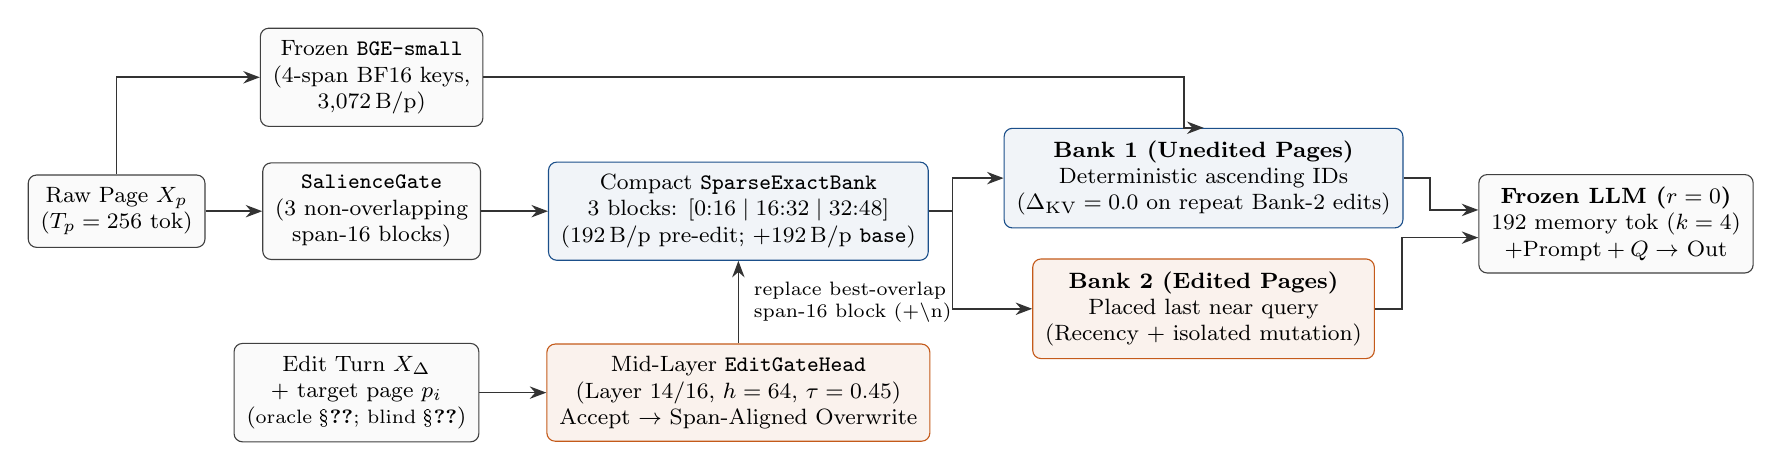
\begin{tikzpicture}[
    node distance=0.65cm and 0.72cm,
    box/.style={draw=black!75, rounded corners=3pt, minimum height=0.82cm, align=center, font=\footnotesize, inner sep=4.5pt, fill=black!2},
    imm/.style={draw=tmlrblue, rounded corners=3pt, minimum height=0.82cm, align=center, font=\footnotesize, inner sep=4.5pt, fill=tmlrblue!6},
    mut/.style={draw=tmlrorange, rounded corners=3pt, minimum height=0.82cm, align=center, font=\footnotesize, inner sep=4.5pt, fill=tmlrorange!8},
    arr/.style={-{Stealth[length=2.1mm]}, semithick, draw=black!80}
]
\node[box] (page) {Raw Page $X_p$\\($T_p=256$ tok)};
\node[box, right=of page] (sg) {\texttt{SalienceGate}\\(3 non-overlapping\\span-16 blocks)};
\node[box, above=0.45cm of sg] (bge) {Frozen \texttt{BGE-small}\\(4-span BF16 keys,\\$3{,}072\,\text{B/p}$)};
\node[imm, right=0.85cm of sg] (bank) {Compact \texttt{SparseExactBank}\\3 blocks: $[0{:}16 \mid 16{:}32 \mid 32{:}48]$\\($192\,\text{B/p}$ pre-edit; $+192\,\text{B/p}$ \texttt{base})};
\node[mut, below=1.05cm of bank] (gate) {Mid-Layer \texttt{EditGateHead}\\(Layer 14/16, $h=64$, $\tau=0.45$)\\Accept $\rightarrow$ Span-Aligned Overwrite};
\node[box, left=0.85cm of gate] (editin) {Edit Turn $X_\Delta$\\+ target page $p_i$\\({\scriptsize oracle \S\ref{sec:gate2_factorial}; blind \S\ref{sec:gate2_e2e}})};
\node[imm, right=0.95cm of bank, yshift=0.42cm] (b1) {\textbf{Bank 1 (Unedited Pages)}\\Deterministic ascending IDs\\($\Delta_{\text{KV}}=0.0$ on repeat Bank-2 edits)};
\node[mut, below=0.38cm of b1] (b2) {\textbf{Bank 2 (Edited Pages)}\\Placed last near query\\(Recency + isolated mutation)};
\node[box, right=0.95cm of b1, yshift=-0.58cm] (llm) {\textbf{Frozen LLM ($r=0$)}\\$192$ memory tok ($k=4$)\\$+ \text{Prompt} + Q \rightarrow$ Out};

\draw[arr] (page.east) -- (sg.west);
\draw[arr] (page.north) |- (bge.west);
\draw[arr] (sg.east) -- (bank.west);
\draw[arr] (editin.east) -- (gate.west);
\draw[arr] (gate.north) -- node[midway, right=2pt, font=\scriptsize, align=left]{replace best-overlap\\span-16 block ($+\backslash\text{n}$)} (bank.south);
\draw[arr] (bge.east) -| ([xshift=-0.25cm]b1.north) -- (b1.north);
\draw[arr] (bank.east) -- ++(0.3,0) |- (b1.west);
\draw[arr] (bank.east) -- ++(0.3,0) |- (b2.west);
\draw[arr] (b1.east) -- ++(0.34,0) |- ([yshift=5pt]llm.west);
\draw[arr] (b2.east) -- ++(0.34,0) |- ([yshift=-5pt]llm.west);
\end{tikzpicture}%
}
\caption{Overview of \texttt{PathBDiscreteMemory} (\texttt{OW-192}; $0$ latent encoder, $0$ $\vect{Z}_{\text{book}}$). Each $256$-token page is indexed by frozen \texttt{BGE-small} 4-span BF16 keys ($3{,}072\,\text{B/p}$) and compressed into three aligned $16$-token spans ($48$ \texttt{int32} IDs $= 192\,\text{B/p}$). Incoming edits $(X_\Delta, p_i)$ accepted by the mid-layer \texttt{ContextualEditGateHead} ($h=64$) overwrite the highest-overlap span-16 block on page $p_i$ with a newline separator. Retrieved pages place unedited pages first (Bank~1) and mutated pages last (Bank~2).}
\label{fig:arch}
\end{figure}

\begin{enumerate}
    \item \textbf{Contiguous Span-16 Salience Extraction:} \texttt{SalienceGate} scores frozen token embeddings and greedily selects $3$ non-overlapping $16$-token windows ($k_{\text{exact}} = 48$ tokens; \texttt{special\_tokens\_in\_bank} $= 0$), falling back to individual top-salience tokens only if fewer than three valid windows exist. Only \texttt{token\_ids: int32} are stored ($48 \times 4 = 192\,\text{B/page}$ pre-edit).
    \item \textbf{Hybrid Dense--Lexical Routing:} Each page stores four BF16 span embeddings from frozen \texttt{BAAI/bge-small-en-v1.5} ($33.36\text{M}$ frozen parameters; $4 \times 384 \times 2 = 3{,}072\,\text{B/page}$). Query routing fuses z-normalized dense cosine logits with unigram/bigram/trigram IDF lexical overlap computed over both pre-edit (\texttt{base\_token\_ids}) and post-edit bank tokens ($w_{\text{sal}} = 1.5$).
    \item \textbf{Supervised Mid-Layer Edit Gate:} \texttt{ContextualEditGateHead} ($h=64$) applies LayerNorm, linear projection to $64$ dimensions, attention + mean pooling, and a 2-layer MLP over frozen Layer-14 (\texttt{Qwen3-1.7B}) or Layer-16 (\texttt{Llama-3.1-8B-Instruct}) hidden states of $X_\Delta$, trained with supervised accept/reject labels on training templates and applied at test time with zero test-time oracle acceptance labels ($p_{\text{acc}} > 0.45$).
    \item \textbf{Span-Aligned Selective Overwrite:} Legacy suffix overwriting ($[48-k_{\text{sticky}}:48]$) frequently split mid-span tokens (producing artifacts such as \texttt{'39Budget'}) while leaving stale facts intact in slots $0{:}16$. Instead, when $p_{\text{acc}} > 0.45$, \texttt{OW-192} partitions the $48$ slots into three aligned span-16 blocks ($[0{:}16], [16{:}32], [32{:}48]$), scores each block by $3\cdot \text{lexical\_overlap\_ratio} + \text{mean\_max\_cosine\_sim}$ against $X_\Delta$ (falling back to $[32{:}48]$ under zero overlap and cosine $< 0.80$), and writes contiguous edit tokens prefixed/padded with a newline token into $1$ block (if $|X_\Delta| \le 15$) or $2$ adjacent blocks ($32$ slots; payloads exceeding $31$ tokens are salience-trimmed). On the first accepted mutation in a book, the bank clones \texttt{token\_ids} into \texttt{base\_token\_ids} ($+192\,\text{B/page}$); subsequent writes to a given page $p_i$ are $O(1)$ in-place tensor writes.
    \item \textbf{Partitioned Two-Bank Ordering:} Given $k_{\text{deep}}$ retrieved pages, unedited pages are ordered first in ascending page-ID order (\textbf{Bank~1}), followed by mutated pages (\textbf{Bank~2}).
\end{enumerate}

\subsection{Exact Parameter, Training, and Storage Accounting}
Table~\ref{tab:accounting} reports exact parameter counts, training budgets, and byte footprints reconciled across both backbones. Storage is $3{,}264\,\text{B/page}$ pre-edit ($3{,}456\,\text{B/page}$ post-edit after cloning \texttt{base\_token\_ids})---$\sim 3.0\times$ larger than bare UTF-8 raw text ($\sim 1{,}083$--$1{,}138\,\text{B/p}$) due to the $3{,}072\,\text{B/p}$ BGE index, $21\%$ smaller than \texttt{bge\_4span\_rag} ($\sim 4{,}155$--$4{,}210\,\text{B/p}$), $4.6\times$--$4.8\times$ smaller than \texttt{LSLC-Full} ($15{,}744$--$15{,}936\,\text{B/p}$), and $8{,}500\times$--$10{,}280\times$ smaller than uncompressed FP16 KV caches ($28.0$--$32.0\,\text{MiB/p}$; pre-edit $8{,}995\times$--$10{,}280\times$, post-edit $8{,}495\times$--$9{,}709\times$). On \texttt{Qwen3-1.7B}, \texttt{SalienceGate} was inherited from the $400$-step frozen-encoder universal stage ($67.05\,\text{s}$, warm-started through two prior stages of $400$ and $250$ steps atop an earlier adapter checkpoint: $1{,}050$ post-adapter steps total) and the $144\text{K}$ edit gate was trained freshly ($24.04\,\text{s}$); on \texttt{Llama-3.1-8B-Instruct}, both modules were trained from scratch in $31.56\,\text{s}$ on a single A100 $40\,\text{GB}$ GPU over splits verified against a forbidden-term audit over evaluation entities and values.

\begin{table}[t]
\centering
\caption{Exact parameter, training, and storage accounting for \texttt{PathBDiscreteMemory} (\texttt{OW-192}) on both frozen BF16 backbones ($r=0$). Storage reports bytes per $256$-token page before and after first-edit \texttt{base\_token\_ids} allocation. On Llama, the gated official repo fell back to the ungated BF16 mirror \texttt{unsloth/Meta-Llama-3.1-8B-Instruct}.}
\label{tab:accounting}
\small
\resizebox{\textwidth}{!}{%
\begin{tabular}{@{}lcc@{}}
\toprule
\textbf{Quantity} & \texttt{Qwen/Qwen3-1.7B} & \texttt{unsloth/Meta-Llama-3.1-8B-Instruct} \\
\midrule
Frozen LLM parameters (\texttt{max\_frozen\_param\_diff} $=0.0$) & $1{,}720{,}574{,}976$ & $8{,}030{,}261{,}248$ \\
Frozen \texttt{bge-small-en-v1.5} router parameters & $33{,}360{,}000$ & $33{,}360{,}000$ \\
\texttt{SalienceGate} trained parameters & $182{,}533$ & $315{,}653$ \\
\texttt{ContextualEditGateHead} ($h=64$) trained parameters & $143{,}874$ (Layer 14) & $279{,}042$ (Layer 16) \\
\texttt{LayeredLatentEncoder} / \texttt{DeltaUpdater} / \texttt{hw\_coord} & $0$ & $0$ \\
\textbf{Total Path B trained parameters (\% of frozen LLM)} & $\mathbf{326{,}407}$ ($0.019\%$) & $\mathbf{594{,}695}$ ($0.0074\%$) \\
Checkpoint size (\texttt{.safetensors}) & $1.25\,\text{MiB}$ ($1{,}307{,}884\,\text{B}$) & $2.27\,\text{MiB}$ ($2{,}381{,}052\,\text{B}$) \\
Training wall-clock (A100 40GB) & $67.05\,\text{s}$ (stage~2) $+ 24.04\,\text{s}$ (Gate) & $31.56\,\text{s}$ (from scratch) \\
\midrule
Path B storage (pre-edit $\rightarrow$ post-edit \texttt{base} clone) & $3{,}264 \rightarrow 3{,}456\,\text{B/p}$ & $3{,}264 \rightarrow 3{,}456\,\text{B/p}$ \\
Reference: BM25 UTF-8 / BGE-4span RAG / FP16 KV & $1{,}083$ / $4{,}155\,\text{B/p}$ / $28.0\,\text{MiB/p}$ & $1{,}138$ / $4{,}210\,\text{B/p}$ / $32.0\,\text{MiB/p}$ \\
\bottomrule
\end{tabular}%
}
\end{table}

% ===========================================================================
\section{Task-Dependent Diagnostics of Short-Budget Latent Prefixes}
\label{sec:diag}
% ===========================================================================

Before isolating discrete write policies, we characterize the empirical behavior of our co-trained input-space continuous latent prefix ($\vect{Z}_{\text{book}}$ + $\Delta\vect{Z}$) under short adapter budgets: the $1{,}050$-step ($400+250+400$ post-adapter, initialized from an earlier adapter release) \texttt{Qwen3-1.7B} \texttt{LSLC-Full} checkpoint ($41.51\text{M}$ total adapter parameters, $31.40\text{M}$ trained in the final frozen-encoder stage) and a $120$-step cross-family probe on \texttt{Llama-3.1-8B-Instruct} ($109.66\text{M}$ adapter parameters, loss $6.38 \rightarrow 3.52$, $88.8\,\text{s}$ combined train + eval).

\subsection{5-Cell Iso-Token Masked-Old Edit Probe}
Leaving the superseded value in \texttt{SparseExactBank} (\texttt{bank\_OFF} = un-updated bank) cannot separate whether the frozen decoder ignores $\Delta\vect{Z}$ vs.\ is outvoted by an explicit stale token. We therefore evaluate a $5$-cell iso-token ablation ($298$ active memory tokens in every arm, all retaining the \texttt{LSLC-Full} latent prefix architecture; $N=48$: $24$ verbatim edits covering $8$ unique target answers repeated $3\times$ each, plus $24$ implicit yes/no edits) that adds \texttt{deltaZ\_ON\_bank\_masked\_old}: replacing stale answer tokens on the target page with neutral filler (mean $3.625$ tokens masked on \texttt{Qwen3-1.7B} verbatim and $2.67$ on \texttt{Llama-3.1-8B-Instruct} verbatim, where $2/24$ episodes had $0$ matching tokens masked; $0.0$ on implicit where \texttt{old\_answer} is not supplied).

\begin{table}[t]
\centering
\caption{5-cell iso-token masked-old edit probe ($298$ active memory tokens in all arms; $N=24$ verbatim, $N=24$ implicit). On \texttt{Llama-3.1-8B-Instruct} \texttt{bank\_ON}, the model emits concise unitless numbers (e.g., \texttt{"45"} for \texttt{"45 days"}); both strict match and manually verified numeric value-match are reported. \texttt{bank\_OFF} retains the un-updated bank.}
\label{tab:5cell}
\small
\resizebox{\textwidth}{!}{%
\begin{tabular}{@{}lcccc@{}}
\toprule
\textbf{Arm ($298$ memory tok)} & \textbf{Qwen3 Verb.} & \textbf{Qwen3 Impl.} & \textbf{Llama-8B Verb. (Strict / Value)} & \textbf{Llama-8B Impl.} \\
\midrule
\texttt{deltaZ\_ON\_bank\_ON} & $\mathbf{1.000}$ ($24/24$) & $0.917$ ($22/24$) & $0.417$ ($10/24$) / $\mathbf{1.000}$ ($24/24$) & $0.833$ ($20/24$) \\
\texttt{deltaZ\_OFF\_bank\_ON} & $\mathbf{1.000}$ ($24/24$) & $0.917$ ($22/24$) & $0.500$ ($12/24$) / $\mathbf{1.000}$ ($24/24$) & $\mathbf{0.875}$ ($21/24$) \\
\texttt{deltaZ\_ON\_bank\_masked\_old} & $\mathbf{0.000}$ ($0/24$) & $0.500$ ($12/24$) & $\mathbf{0.000}$ ($0/24$) / $\mathbf{0.000}$ ($0/24$) & $0.667$ ($16/24$) \\
\texttt{deltaZ\_ON\_bank\_OFF} & $0.000$ ($0/24$) & $0.500$ ($12/24$) & $0.000$ ($0/24$) / $0.000$ ($0/24$) & $0.667$ ($16/24$) \\
\texttt{deltaZ\_OFF\_bank\_OFF} & $0.000$ ($0/24$) & $0.458$ ($11/24$) & $0.042$ ($1/24$) / $0.042$ ($1/24$) & $0.708$ ($17/24$) \\
\bottomrule
\end{tabular}%
}
\end{table}

Table~\ref{tab:5cell} shows that with these checkpoints and prompts, the frozen decoder produces $\mathbf{0/24}$ edited verbatim answers in \texttt{deltaZ\_ON\_bank\_masked\_old} on both \texttt{Qwen3-1.7B} (emitting numeric guesses such as \texttt{"120"} or \texttt{"1000000"}) and \texttt{Llama-3.1-8B-Instruct} (emitting WikiText/degenerate strings such as \texttt{",,"}, \texttt{"0"}, and \texttt{"M @-@ 82"}), identical to \texttt{deltaZ\_ON\_bank\_OFF} ($0$ vs.\ $0$, exact McNemar $p=1.0$). Decoding failure does not by itself prove zero information inside $\Delta\vect{Z}$, but shows that the frozen decoder does not read out verbatim edits without discrete bank updates. Enabling $\Delta\vect{Z}$ alongside an updated bank gives $0.0\pp$ change on \texttt{Qwen3-1.7B} and $-6.25\pp$ overall ($0$ vs.\ $3$, $p=0.25$) on \texttt{Llama-3.1-8B-Instruct}.

\subsection{Cross-Task Latent Prefix Interaction}
Crucially, Figure~\ref{fig:latent_interaction} summarizes four diagnostic pairs (comparing bank-only / exact-only baselines against latent-only masked-old readout or $+\vect{Z}_{\text{book}}$) revealing a \emph{task-dependent interaction} rather than uniform collapse:
\begin{itemize}
    \item \textbf{Severe Degradation on Coding and Continuation Perplexity:} On locked-page $65$-file Python API migration (\texttt{Qwen3-1.7B}, $N=24$, Section~\ref{sec:coding}), adding $\vect{Z}_{\text{book}}$ drops \texttt{pass@1} from $20/24$ ($83.3\%$, \texttt{lslc\_exact\_only\_k4}) to $\mathbf{1/24}$ ($4.2\%$, \texttt{lslc\_full\_k4}; $0$ vs.\ $19$, $p=3.81\times 10^{-6}$). On $4\text{K}$ \texttt{WikiText-2}~\citep{merity2017wikitext} continuation perplexity, \texttt{LSLC-Full} increases PPL from $25.91$ (\texttt{OW-192}) to $\mathbf{39.86}$ ($\Delta=+13.94$, $N=16$) on \texttt{Qwen3-1.7B} and from $14.08$ to $\mathbf{17.89}$ ($\Delta=+3.81$, $N=15$) on \texttt{Llama-3.1-8B-Instruct} (noting that prefix length, assembly, and retrieved page sets can also differ between pipelines).
    \item \textbf{Mixed Results on Static Retrieval:} On $4\text{K}$ \texttt{RULER-style} QA (\texttt{Qwen3-1.7B}, $N=48$), \texttt{LSLC-Full} scores $50.0\%$ vs.\ $56.3\%$ for \texttt{OW-192} ($2$ vs.\ $5$, $p=0.45$, n.s.), whereas on $16\text{K}$/$32\text{K}$ \texttt{RULER-style} QA (in the unified \texttt{Qwen3-1.7B} RULER/profile run), \texttt{LSLC-Full} scored $71.7\%$/$66.7\%$ vs.\ $68.3\%$/$65.0\%$ for \texttt{OW-192}.
    \item \textbf{Positive Assist Under Legacy Suffix Overwrite:} On \texttt{Gate-2} (\texttt{Qwen3-1.7B}, $N=600$, seeds $2029$--$2031$) under the legacy suffix-overwrite policy ($[48-k_{\text{sticky}}:48]$), \texttt{lslc\_full} ($383/600 = 63.8\%$) outperforms \texttt{lslc\_exact\_only} ($351/600 = 58.5\%$; $+5.33\pp$, $53$ vs.\ $21$, exact $p=2.56\times 10^{-4}$, cluster-bootstrap $95\%$ CI $[+1.45\%, +9.46\%]$), with pooled gains of $+8.7\pp$ on accepted ($60.0\%$ vs.\ $51.3\%$) and $+12.7\pp$ on rejected ($54.7\%$ vs.\ $42.0\%$) queries ($+14.7\pp$ and $+22.7\pp$ on budget queries alone; $+2.7\pp$ and $+2.7\pp$, n.s., on symbolic). Replacing legacy suffix overwriting with span-aligned overwrite (\texttt{OW-192}, Section~\ref{sec:gate2}) reaches $76.7\%$, surpassing legacy \texttt{lslc\_full} by $+12.8\pp$ ($99$ vs.\ $22$, $p=7.41\times 10^{-13}$) without the $41.5\text{M}$-parameter \texttt{LSLC-Full} adapter suite ($10.1\text{M}$ encoder + $22.9\text{M}$ projector + updater/router) or its coding/PPL penalties.
\end{itemize}

\begin{figure}[t]
\centering
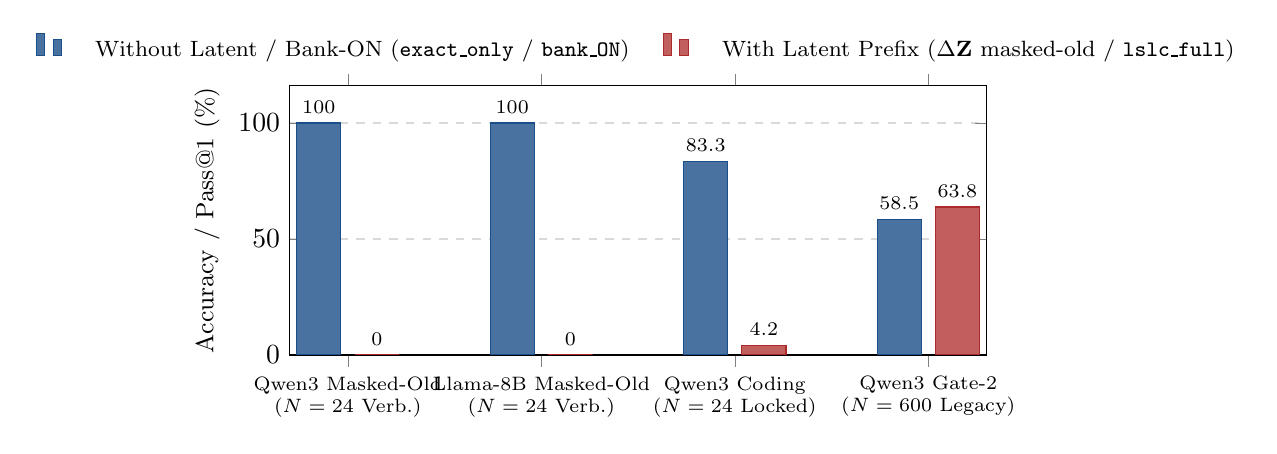
\begin{tikzpicture}
\begin{axis}[
    ybar=5pt,
    bar width=16pt,
    width=0.86\textwidth,
    height=5.0cm,
    ymin=0, ymax=116,
    ylabel={Accuracy / Pass@1 (\%)},
    symbolic x coords={qmask, lmask, qcod, qg2},
    xticklabels={{Qwen3 Masked-Old\\($N=24$ Verb.)}, {Llama-8B Masked-Old\\($N=24$ Verb.)}, {Qwen3 Coding\\($N=24$ Locked)}, {Qwen3 Gate-2\\($N=600$ Legacy)}},
    xtick=data,
    xticklabel style={font=\scriptsize, align=center},
    ylabel style={font=\small},
    legend style={at={(0.5,1.05)}, anchor=south, legend columns=2, column sep=10pt, font=\footnotesize, draw=none},
    nodes near coords,
    nodes near coords style={font=\scriptsize, above},
    ymajorgrids=true,
    grid style={dashed, gray!30}
]
\addplot[fill=tmlrblue!80, draw=tmlrblue] coordinates {
    (qmask, 100.0) (lmask, 100.0) (qcod, 83.3) (qg2, 58.5)
};
\addplot[fill=tmlrred!75, draw=tmlrred] coordinates {
    (qmask, 0.0) (lmask, 0.0) (qcod, 4.2) (qg2, 63.8)
};
\legend{Without Latent / Bank-ON (\texttt{exact\_only} / \texttt{bank\_ON}), With Latent Prefix ($\Delta\mathbf{Z}$ masked-old / \texttt{lslc\_full})}
\end{axis}
\end{tikzpicture}
\caption{Strictly matched pairwise comparison of the short-budget co-trained latent prefix across four evaluations (each bar corresponds directly to a measured arm; no unmeasured proxy bars are plotted). For masked-old verbatim readout (first two groups), bars compare \texttt{deltaZ\_OFF\_bank\_ON} (value-EM $24/24$) against \texttt{deltaZ\_ON\_bank\_masked\_old} ($0/24$). Adding $\vect{Z}_{\text{book}}$ collapses locked-page Python coding ($83.3\% \rightarrow 4.2\%$) yet improves legacy suffix-overwrite \texttt{Gate-2} ($58.5\% \rightarrow 63.8\%$).}
\label{fig:latent_interaction}
\end{figure}

% ===========================================================================
\section{Controlled Study: In-Place Span Overwrite vs.\ Append (\texttt{Gate-2})}
\label{sec:gate2}
% ===========================================================================

To evaluate write policies (overwrite vs.\ append), page ordering (\texttt{edited\_last} vs.\ \texttt{page\_id\_asc}), and memory compression ($192$ memory tokens vs.\ $\sim 1{,}030$--$1{,}062$ raw memory tokens), we use \texttt{AdversarialLivingBookDataset} (\texttt{Gate-2}): $16$-page synthetic documents ($4{,}096$ tokens) mixing held-out budget revisions ($k=3$ edits) and symbolic topology revisions ($k=5$ edits), queried equally across four query types (\texttt{accepted\_override}, \texttt{rejected\_proposal}, \texttt{neighbor\_preservation}, and \texttt{randomized\_static\_retention}). Each episode mutates one project page, while static policies, the target project, and the neighbor project reside on separate pages. All arms share the exact same $2$-shot format prefix (\texttt{\_FAIR\_G2\_FEWSHOT\_PREFIX}, Appendix~\ref{app:prompt}; note that its demo answer \texttt{"40M"} overlaps the $26$--$40\text{M}$ initial budget range identically across arms).

\subsection{Locked-Pages \& Locked-Order 2x4 Factorial}
\label{sec:gate2_factorial}
In end-to-end runs, different write policies alter lexical retrieval scores and prefix page order. To evaluate all four write policies conditionally on identical retrieved pages and identical page orders ($N=200$ per backbone: seed $2029$ on \texttt{Qwen3-1.7B}, seed $2026$ on \texttt{Llama-3.1-8B-Instruct}), our factorial runs \texttt{OW-192}'s post-edit hybrid router \emph{once} per episode to lock $4$ identical page IDs across all $8$ arms (verified across all $3{,}200$ arm--episode records with $0$ page-ID or ordering mismatches). All four policies receive the same oracle edit page address $p_i$ during ingestion and identical mid-layer edit-gate decisions ($450$ TP, $350$ TN, $0$ FP, $0$ FN on both backbones), crossing $2$ page orders (\texttt{edited\_last} vs.\ \texttt{page\_id\_asc}; note that the two rules coincide on $77/200$ Qwen and $75/200$ Llama episodes, where the edited page either already has the highest ID---$49/77$ Qwen, $43/75$ Llama---or is not among the $4$ locked pages---$28/77$ Qwen, $32/75$ Llama) with $4$ write policies:
\begin{enumerate}
    \item \texttt{Raw-App} (\texttt{raw\_text\_append}): gated raw text appending accepted turns prefixed with literal \texttt{"Update: "} at page end ($\sim 1{,}060$ memory tok; without an explicit prompt instruction stating that later updates supersede earlier lines);
    \item \texttt{Raw-OW} (\texttt{raw\_text\_overwrite}): a \emph{schema-aware rule-based} raw-text heuristic (non-oracle with respect to gold answers or sentence IDs within the given page $p_i$, but tailored with \texttt{Gate-2} stopword lists, \texttt{RECORD:}/\texttt{POLICY:} guards, and entity-overlap scoring) replacing matching prior lines in place ($\sim 1{,}030$ memory tok; returning \texttt{replaced=True} on $450/450$ accepted turns, though full post-edit text diffs are not logged and same-page neighbor protection is untested because neighbor projects sit on separate pages);
    \item \texttt{App-192} (\texttt{standalone\_append\_192tok}): $192$-token bank preserving slots $0{:}16$, inserting a newline separator, keeping the last $31$ tokens of accepted edit history (\texttt{app\_toks[-31:]}), and refilling any remaining capacity from the initial bank (when edits fill the tail, the other two salience blocks are displaced);
    \item \texttt{OW-192} (\texttt{standalone\_overwrite\_192tok}): \texttt{PathBDiscreteMemory} with Span-Aligned Selective Overwrite.
\end{enumerate}

\begin{table}[t]
\centering
\caption{Locked-page, locked-order $2\times 4$ factorial on \texttt{Gate-2} ($N=200$/backbone; $4$ identical post-edit \texttt{OW-192} router pages, shared oracle $p_i$, and identical edit-gate decisions across all $8$ arms). Primary metric is \texttt{Norm-EM} (identical to \texttt{strict\_em} on all $3{,}200$ rows); \texttt{W2N-EM} in parentheses adds word-to-number canonicalization. Unrounded exact McNemar $p$-values are Holm-adjusted over $m=12$ contrasts per metric per backbone; cluster $95\%$ CIs ($B=2{,}000$, $C=52$ Qwen / $57$ Llama) are nominal per contrast.}
\label{tab:factorial}
\small
\resizebox{\textwidth}{!}{%
\begin{tabular}{@{}lccccc@{}}
\toprule
\textbf{Write Policy (Locked 4 Pages)} & \textbf{Qwen3 \texttt{ed\_last}} & \textbf{Qwen3 \texttt{id\_asc}} & \textbf{Llama-8B \texttt{ed\_last}} & \textbf{Llama-8B \texttt{id\_asc}} & \textbf{Mem.\ Tok} \\
\midrule
\texttt{Raw-App} (\texttt{raw\_text\_append}) & $48.0\%$ ($54.0\%$) & $45.5\%$ ($52.0\%$) & $70.5\%$ ($76.5\%$) & $65.5\%$ ($72.0\%$) & $1{,}059$--$1{,}062$ \\
\texttt{Raw-OW} (schema-aware rule-based) & $71.0\%$ ($77.0\%$) & $60.5\%$ ($66.5\%$) & $\mathbf{89.0\%}$ ($\mathbf{95.0\%}$) & $\mathbf{85.5\%}$ ($\mathbf{92.0\%}$) & $1{,}029$--$1{,}030$ \\
\texttt{App-192} ($31$-tok rolling tail) & $59.5\%$ ($64.5\%$) & $55.5\%$ ($60.5\%$) & $76.0\%$ ($80.5\%$) & $70.0\%$ ($74.5\%$) & $192$ \\
\texttt{OW-192} (Path B span overwrite) & $\mathbf{74.5\%}$ ($\mathbf{79.5\%}$) & $\mathbf{66.5\%}$ ($\mathbf{71.5\%}$) & $85.5\%$ ($90.0\%$) & $79.0\%$ ($83.5\%$) & $\mathbf{192}$ \\
\midrule
\multicolumn{6}{@{}l@{}}{\textit{Paired contrasts on \texttt{Norm-EM} (discordant wins, unrounded Holm $p_{\text{H}}$, nominal cluster $95\%$ CI in pp; exact cluster sign-flip $p_{\text{sf,H}}$ in text):}} \\
\texttt{OW-192} vs.\ \texttt{App-192} (\texttt{ed\_last}) & \multicolumn{2}{l}{$+15.0$ ($32$--$2$, $p_{\text{H}}=6.24\times 10^{-7}$, $[+8.7,+21.7]$)} & \multicolumn{3}{l}{$+9.5$ ($22$--$3$, $p_{\text{H}}=1.25\times 10^{-3}$, $[+2.8,+16.3]$)} \\
\texttt{OW-192} vs.\ \texttt{App-192} (\texttt{id\_asc}) & \multicolumn{2}{l}{$+11.0$ ($27$--$5$, $p_{\text{H}}=6.78\times 10^{-4}$, $[+4.9,+17.8]$)} & \multicolumn{3}{l}{$+9.0$ ($22$--$4$, $p_{\text{H}}=3.73\times 10^{-3}$, $[+2.3,+15.8]$)} \\
\texttt{Raw-OW} vs.\ \texttt{Raw-App} (\texttt{ed\_last}/\texttt{id\_asc}) & \multicolumn{2}{l}{$+23.0/+15.0$ ($p_{\text{H}}\le 1.11\times 10^{-5}$)} & \multicolumn{3}{l}{$+18.5/+20.0$ ($p_{\text{H}}\le 2.15\times 10^{-10}$)} \\
\texttt{OW-192} vs.\ \texttt{Raw-OW} (\texttt{Norm-EM}) & \multicolumn{2}{l}{$+3.5/+6.0$ ($p_{\text{H}}=0.453/0.091$, $[-2.8,+10.3]/[-0.4,+13.4]$)} & \multicolumn{3}{l}{$-3.5/-6.5$ ($p_{\text{H}}=0.118/0.052$, $[-7.7,+0.5]/[-13.5,-0.9]$)} \\
\texttt{OW-192} vs.\ \texttt{Raw-OW} (\texttt{W2N-EM}) & \multicolumn{2}{l}{$+2.5/+5.0$ ($p_{\text{H}}=0.775/0.302$, $[-3.8,+9.3]/[-1.5,+12.6]$)} & \multicolumn{3}{l}{$-5.0/-8.5$ ($p_{\text{H}}=0.105/\mathbf{0.0116}$, $[-9.5,-1.0]/[-16.0,-2.6]$)} \\
Order \texttt{ed\_last} vs.\ \texttt{id\_asc} (\texttt{OW-192}) & \multicolumn{2}{l}{$+8.0$ ($17$--$1$, $p_{\text{H}}=7.25\times 10^{-4}$, $[+3.7,+13.2]$)} & \multicolumn{3}{l}{$+6.5$ ($15$--$2$, $p_{\text{H}}=0.0118$, $[+1.9,+12.1]$)} \\
\bottomrule
\end{tabular}%
}
\end{table}

\begin{figure}[t]
\centering
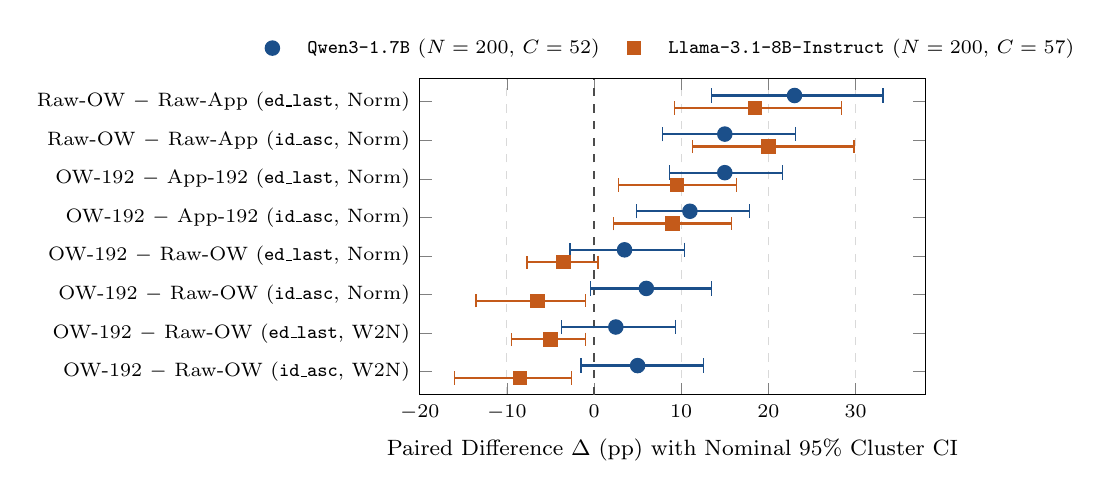
\begin{tikzpicture}
\begin{axis}[
    width=0.66\textwidth,
    height=5.6cm,
    xmin=-20, xmax=38,
    ymin=0.4, ymax=8.6,
    ytick={1,2,3,4,5,6,7,8},
    yticklabels={
        {OW-192 $-$ Raw-OW (\texttt{id\_asc}, W2N)},
        {OW-192 $-$ Raw-OW (\texttt{ed\_last}, W2N)},
        {OW-192 $-$ Raw-OW (\texttt{id\_asc}, Norm)},
        {OW-192 $-$ Raw-OW (\texttt{ed\_last}, Norm)},
        {OW-192 $-$ App-192 (\texttt{id\_asc}, Norm)},
        {OW-192 $-$ App-192 (\texttt{ed\_last}, Norm)},
        {Raw-OW $-$ Raw-App (\texttt{id\_asc}, Norm)},
        {Raw-OW $-$ Raw-App (\texttt{ed\_last}, Norm)}
    },
    yticklabel style={font=\scriptsize},
    xlabel={Paired Difference $\Delta$ (pp) with Nominal 95\% Cluster CI},
    xlabel style={font=\footnotesize},
    tick label style={font=\scriptsize},
    xmajorgrids=true,
    grid style={dashed, gray!30},
    legend style={at={(0.5,1.03)}, anchor=south, legend columns=2, column sep=8pt, font=\scriptsize, draw=none}
]
\draw[black!70, thick, dashed] (axis cs:0,0.4) -- (axis cs:0,8.6);

% Qwen3-1.7B (offset +0.16) — exact asymmetric cluster-bootstrap 95% CIs
\addplot[only marks, mark=*, mark size=2.6pt, color=tmlrblue,
    error bars/.cd, x dir=both, x explicit, error bar style={thick, color=tmlrblue}]
table[x=x, y=y, x error minus=xm, x error plus=xp] {
x     y     xm    xp
23.0  8.16  9.55  10.15
15.0  7.16  7.12  8.13
15.0  6.16  6.35  6.65
11.0  5.16  6.14  6.79
3.5   4.16  6.26  6.83
6.0   3.16  6.40  7.44
2.5   2.16  6.28  6.81
5.0   1.16  6.50  7.57
};
% Llama-3.1-8B-Instruct (offset -0.16) — exact asymmetric cluster-bootstrap 95% CIs
\addplot[only marks, mark=square*, mark size=2.4pt, color=tmlrorange,
    error bars/.cd, x dir=both, x explicit, error bar style={thick, color=tmlrorange}]
table[x=x, y=y, x error minus=xm, x error plus=xp] {
x     y     xm    xp
18.5  7.84  9.31  9.92
20.0  6.84  8.72  9.82
9.5   5.84  6.70  6.83
9.0   4.84  6.73  6.81
-3.5  3.84  4.19  3.96
-6.5  2.84  7.04  5.56
-5.0  1.84  4.47  4.04
-8.5  0.84  7.46  5.88
};
\legend{{\texttt{Qwen3-1.7B} ($N=200$, $C=52$)}, {\texttt{Llama-3.1-8B-Instruct} ($N=200$, $C=57$)}}
\end{axis}
\end{tikzpicture}
\caption{Paired accuracy differences ($\Delta$ in pp) and nominal $95\%$ cluster-bootstrap CIs for the \texttt{Gate-2} $2\times 4$ factorial (Table~\ref{tab:factorial}). Both raw-text and $192$-token overwrite beat append with every CI strictly above zero. Against schema-aware \texttt{Raw-OW}, \texttt{OW-192} shows positive point estimates on \texttt{Qwen3-1.7B} (CIs crossing $0$), but is outperformed on \texttt{Llama-3.1-8B-Instruct} under \texttt{id\_asc} and W2N-EM (CIs strictly below $0$).}
\label{fig:factorial}
\end{figure}

Table~\ref{tab:factorial} and Figure~\ref{fig:factorial} isolate three empirical findings:
\begin{enumerate}
    \item \textbf{Overwrite vs.\ Rolling-Tail Append under Fixed Memory Budget:} On both page orders, \texttt{OW-192} outperforms \texttt{App-192} by $+11.0\pp$ to $+15.0\pp$ on \texttt{Qwen3-1.7B} ($p_{\text{Holm}} \le 6.78\times 10^{-4}$) and $+9.0\pp$ to $+9.5\pp$ on \texttt{Llama-3.1-8B-Instruct} ($p_{\text{Holm}} \le 3.73\times 10^{-3}$), with all four nominal cluster CIs strictly positive. On \texttt{Llama-3.1-8B-Instruct} (\texttt{ed\_last}), the $+9.5\pp$ gain concentrates entirely on mutable queries ($+18\pp$ \texttt{accepted\_override}, $+20\pp$ \texttt{rejected\_proposal}, $0\pp$ neighbor/static). Because \texttt{App-192} retains slots $0{:}16$ while truncating edit history into a $31$-token rolling tail, this contrast reflects the joint effect of stale-fact removal, tail truncation, and block placement. As an inference sensitivity check, an exact cluster-level sign-flip test (Holm-adjusted over $m=12$) preserves significance on \texttt{Qwen3-1.7B} ($p_{\text{sf,H}} = 0.0004$ \texttt{ed\_last}, $0.0146$ \texttt{id\_asc}) but yields $p_{\text{sf,H}} = 0.1265$ and $0.1304$ on single-seed \texttt{Llama-3.1-8B-Instruct}, indicating that Holm-corrected inference strength on Llama depends on the statistical unit. On uncompressed raw text, \texttt{Raw-OW} vs.\ \texttt{Raw-App} yields $+15.0\pp$ to $+23.0\pp$ ($p_{\text{sf,H}} \le 0.003$ on both backbones).
    \item \textbf{Backbone-Divergent Outcome vs.\ Schema-Aware \texttt{Raw-OW}:} On \texttt{Qwen3-1.7B}, \texttt{OW-192} ($192$ memory tok) scores $+3.5\pp$ to $+6.0\pp$ higher than \texttt{Raw-OW} ($1{,}030$ memory tok, $p_{\text{Holm}} = 0.453 / 0.091$, CIs crossing $0$). On \texttt{Llama-3.1-8B-Instruct}, however, \texttt{OW-192} is \emph{outperformed} by \texttt{Raw-OW}: $-3.5\pp$ (\texttt{ed\_last}, $p_{\text{Holm}}=0.118$, CI $[-7.7\%, +0.5\%]$) and $-6.5\pp$ (\texttt{id\_asc}, raw $p=0.0146$, $p_{\text{Holm}}=0.0518$, CI $[-13.5\%, -0.9\%]$) on Norm-EM, widening to $-5.0\pp$ (\texttt{ed\_last}, $p_{\text{Holm}}=0.105$, CI $[-9.5\%, -1.0\%]$) and $-8.5\pp$ (\texttt{id\_asc}, $6$--$23$, $p_{\text{Holm}}=0.0116$, CI $[-16.0\%, -2.6\%]$) on W2N-EM. On mutable queries alone (\texttt{accepted} $+$ \texttt{rejected}, $N=100$), \texttt{Raw-OW} leads \texttt{OW-192} by $99\%$ vs.\ $90\%$ (\texttt{ed\_last}) and $91\%$ vs.\ $78\%$ (\texttt{id\_asc}). Meanwhile, \texttt{OW-192} still exceeds \texttt{Raw-App} by $+13.5\pp$ to $+15.0\pp$ ($p_{\text{Holm}} \le 6.68\times 10^{-5}$, $p_{\text{sf,H}} \le 0.011$) at $5.4\times$ fewer memory tokens. Because the two backbones differ in model family, tokenizer, adapter training, and evaluation seed, we report this cross-backbone divergence without attributing it solely to parameter scale.
    \item \textbf{Order Effect and Policy Interaction:} Placing mutated pages last (\texttt{edited\_last}) raises \texttt{OW-192} by $+8.0\pp$ on \texttt{Qwen3-1.7B} ($p_{\text{Holm}}=7.25\times 10^{-4}$) and $+6.5\pp$ on \texttt{Llama-3.1-8B-Instruct} ($p_{\text{Holm}}=0.0118$). Order and policy are \emph{not} strictly additive: on \texttt{Qwen3-1.7B} raw text, the overwrite--append gap shifts from $+15.0\pp$ (\texttt{id\_asc}) to $+23.0\pp$ (\texttt{ed\_last}), a difference-in-differences of $+8.0\pp$ (nominal cluster CI $[+2.9\%, +13.0\%]$; bank interaction $+4.0\pp$, CI $[-0.5\%, +8.4\%]$).
\end{enumerate}

\subsection{End-to-End Multi-Seed Policies, Blind Edit Routing, and Latency Amortization}
\label{sec:gate2_e2e}
Table~\ref{tab:gate2_e2e} summarizes the end-to-end \texttt{Gate-2} comparison across $3$ seeds on \texttt{Qwen3-1.7B} ($2029$--$2031$, $N=600$ pooled; legacy seeds $2026$--$2028$ in Appendix~\ref{app:legacy}) and $1$ seed on \texttt{Llama-3.1-8B-Instruct} ($2026$, $N=200$). \textbf{Seed overlap disclosure:} the $N=200$ factorial in Table~\ref{tab:factorial} shares seed $2029$ (\texttt{Qwen3-1.7B}, $200/600$ episodes) and seed $2026$ (\texttt{Llama-3.1-8B-Instruct}, $200/200$ episodes) with Table~\ref{tab:gate2_e2e}, yielding identical predictions for the \texttt{edited\_last} $192$-token bank arms. Across the $N=400$ \emph{genuinely fresh} \texttt{Qwen3-1.7B} episodes (seeds $2030 + 2031$), \texttt{OW-192} replicates the exact $+15.0\pp$ margin over \texttt{App-192}: $311/400$ ($77.75\%$) vs.\ $251/400$ ($62.75\%$), $66$--$6$, exact $p=7.26\times 10^{-14}$, nominal cluster CI $[+9.34\%, +20.76\%]$ ($C=56$).

\begin{table}[t]
\centering
\caption{End-to-end \texttt{Gate-2} policy evaluation: \texttt{Qwen3-1.7B} ($N=600$, seeds $2029$--$2031$; seed $2029$ overlaps Table~\ref{tab:factorial}) and single-seed \texttt{Llama-3.1-8B-Instruct} ($N=200$, seed $2026$, overlapping Table~\ref{tab:factorial}). Cycle totals are rounded from unrounded per-episode component means.}
\label{tab:gate2_e2e}
\small
\setlength{\tabcolsep}{4pt}
\resizebox{\textwidth}{!}{%
\begin{tabular}{@{}lcccccc@{}}
\toprule
\textbf{System} & \textbf{Norm-EM} & \textbf{W2N-EM} & \textbf{Acc / Rej / Nbr / Stat} & \textbf{Mem.\ Tok} & \textbf{\texttt{enc/ed/q} (ms)} & \textbf{Cycle (ms)} \\
\midrule
\multicolumn{7}{@{}l@{}}{\textit{\texttt{Qwen/Qwen3-1.7B} (Pooled $N=600$, seeds $2029$--$2031$; $C=57$ clusters; $0$ observed \texttt{'39Budget'} edit artifacts on \texttt{OW-192})}} \\
\texttt{bm25\_rag\_append\_errata} & $54.0\%$ & $58.5\%$ & $30.7 / 38.0 / \mathbf{100} / 47.3$ & $1{,}083$ & $2.0 / 0.1 / 220.6$ & $222.6$ \\
\texttt{gated\_bm25\_rag} (FAR/FRR $0/0$) & $50.7\%$ & $55.7\%$ & $26.7 / 28.7 / \mathbf{100} / 47.3$ & $1{,}056$ & $2.0 / 173.9 / 217.5$ & $393.3$ \\
\texttt{raw\_text\_same\_pages\_k4}* & $44.5\%$ & $49.5\%$ & $15.3 / 22.7 / 98.7 / 41.3$ & $1{,}058$ & $29.8 / 174.7 / 223.1$ & $427.6$ \\
\texttt{App-192} (\texttt{standalone\_append\_192tok}) & $61.7\%$ & $65.5\%$ & $62.0 / 48.7 / 94.7 / 41.3$ & $192$ & $29.3 / 175.1 / 218.2$ & $422.5$ \\
\textbf{\texttt{OW-192}} (\texttt{PathBDiscreteMemory}) & $\mathbf{76.7\%}$ & $\mathbf{81.0\%}$ & $\mathbf{84.7} / \mathbf{85.3} / 93.3 / 43.3$ & $\mathbf{192}$ & $29.3 / 186.2 / 219.2$ & $434.7$ \\
\texttt{lslc\_exact\_only} (legacy suffix) & $58.5\%$ & $62.2\%$ & $51.3 / 42.0 / 96.7 / 44.0$ & $192$ & $38.3 / 205.1 / 234.0$ & $477.3$ \\
\texttt{lslc\_full} (legacy suffix $+ \vect{Z}_{\text{book}}$) & $63.8\%$ & $67.3\%$ & $60.0 / 54.7 / 96.7 / 44.0$ & $306$ & $38.3 / 204.8 / 226.2$ & $469.3$ \\
\midrule
\multicolumn{7}{@{}l@{}}{\textit{\texttt{unsloth/Meta-Llama-3.1-8B-Instruct} BF16 ($N=200$, seed $2026$; $C=57$ clusters; FAR/FRR $0.000/0.000$ on all gated arms)}} \\
\texttt{bm25\_rag\_append\_errata} & $77.0\%$ & $81.5\%$ & $62 / 84 / \mathbf{100} / 62$ & $1{,}081$ & $2.1 / 0.1 / 248.5$ & $250.7$ \\
\texttt{gated\_bm25\_rag} & $69.0\%$ & $73.5\%$ & $58 / 56 / \mathbf{100} / 62$ & $1{,}055$ & $2.0 / 159.4 / 244.2$ & $405.6$ \\
\texttt{raw\_text\_same\_pages\_k4}* & $61.5\%$ & $68.0\%$ & $38 / 50 / \mathbf{100} / 58$ & $1{,}056$ & $31.4 / 159.4 / 247.6$ & $438.3$ \\
\texttt{App-192} (\texttt{standalone\_append\_192tok}) & $76.0\%$ & $80.5\%$ & $72 / 70 / \mathbf{100} / 62$ & $192$ & $29.4 / 160.6 / 186.1$ & $376.0$ \\
\textbf{\texttt{OW-192}} (\texttt{PathBDiscreteMemory}) & $\mathbf{85.5\%}$ & $\mathbf{90.0\%}$ & $\mathbf{90} / \mathbf{90} / \mathbf{100} / 62$ & $\mathbf{192}$ & $29.4 / 172.5 / \mathbf{185.6}$ & $387.5$ \\
\bottomrule
\end{tabular}%
}
\vspace{2pt}
\parbox{\textwidth}{\footnotesize *In the end-to-end runner, \texttt{raw\_text\_same\_pages\_k4} routed on the pre-edit bank without \texttt{edited\_last} placement; exact locked-page controls are in Table~\ref{tab:factorial}. Offline cluster-bootstrap $95\%$ CIs ($C=57$, \texttt{seed=2026}): Qwen3 \texttt{OW-192} vs.\ \texttt{App-192} $[+9.8\%, +20.4\%]$ ($p=8.08\times 10^{-21}$), vs.\ BM25 $[+13.5\%, +31.9\%]$ ($p=2.60\times 10^{-27}$); Llama \texttt{OW-192} vs.\ \texttt{App-192} $[+2.8\%, +16.3\%]$ ($p=1.57\times 10^{-4}$), vs.\ BM25 $[+3.1\%, +14.0\%]$ ($p=0.0046$).}
\end{table}

\begin{itemize}
    \item \textbf{\texttt{gated\_bm25\_rag} vs.\ ungated \texttt{bm25\_rag\_append\_errata}:} Adding the $0\%$ FAR/FRR gate to BM25 lowers accuracy by $-3.3\pp$ on \texttt{Qwen3-1.7B} ($15$--$35$, $p=0.0066$) and $-8.0\pp$ on \texttt{Llama-3.1-8B-Instruct} ($4$--$20$, $p=0.00154$). A plausible mechanism visible in the dataset templates is that rejected turns often restate the valid value \texttt{\{old\}} (e.g., \emph{``Planned cutover of \{proj\} from \{old\} toward \{new\} was called off''}), so appending rejected turns may reinforce the gold value near the prompt tail and alter BM25 term rankings, though reinforcement and ranking shifts were not separately ablated.
    \item \textbf{Non-edit regression and static span-boundary splicing on \texttt{Qwen3-1.7B}:} On unmodified \texttt{neighbor\_preservation} queries (\texttt{Qwen3-1.7B}), \texttt{OW-192} drops to $140/150$ ($93.3\%$) vs.\ $150/150$ ($100.0\%$) for BM25 ($0$--$10$, $p=0.00195$). Furthermore, while edit overwriting inserts a newline separator (yielding $0$ observed \texttt{'39Budget'} edit artifacts), static $3\times 16$-token extraction concatenates non-adjacent spans without a separator, causing block-boundary token splicing in $3$ \texttt{Qwen3-1.7B} factorial \texttt{neighbor\_preservation} failures (\texttt{'read-only-rep90'}, \texttt{'read-only-re border'}, \texttt{'read-only-re'}). On \texttt{Llama-3.1-8B-Instruct}, \texttt{App-192} ($76.0\%$) and ungated BM25 ($77.0\%$, $17$--$19$, $p=0.868$) are statistically indistinguishable on this single $N=200$ seed.
    \item \textbf{Blind edit-page routing ($0$ oracle $p_i$):} Replacing oracle target page indices $p_i$ with blind hybrid routing across $720$ edit turns on \texttt{Qwen3-1.7B} ($N=180$, $3$ seeds) yields $91.81\%$ ($661/720$) turn routing accuracy and $127/180$ ($70.6\%$, W2N $76.7\%$) end-to-end accuracy---below oracle $p_i$ on the same $180$ episodes ($135/180 = 75.0\%$, $0$--$8$, $p=0.00781$), above \texttt{bm25\_rag\_append\_errata} ($86/180$, $49$--$8$, $p=2.72\times 10^{-8}$), and numerically above legacy \texttt{lslc\_full} ($114/180$, $29$--$16$, $p=0.0725$). On \texttt{Llama-3.1-8B-Instruct} ($N=60$, $240$ turns), blind routing reaches $94.17\%$ turn accuracy and $54/60$ ($90.0\%$, W2N $93.3\%$) with $0$ discordant episodes vs.\ oracle ($54/60$, $p=1.0$).
    \item \textbf{Query latency vs.\ full write+read cycle:} On \texttt{Llama-3.1-8B-Instruct}, \texttt{OW-192} is $1.34\times$ faster per query ($185.6$ vs.\ $248.5\,\text{ms}$, noting that our BM25 baseline rebuilds its index in the query path), but incurs $199.7\,\text{ms}$ extra encode+edit overhead ($29.4 + 172.5$ vs.\ $2.1 + 0.1\,\text{ms}$), making a single-query cycle slower ($387.5$ vs.\ $250.7\,\text{ms}$). The estimated break-even on \texttt{Llama-3.1-8B-Instruct} is therefore $\mathbf{\ge 4}$ queries per edit episode ($199.7 / 62.9 = 3.17$); on \texttt{Qwen3-1.7B}, per-query latency is nearly identical ($219.2$ vs.\ $220.6\,\text{ms}$), so write overhead does not amortize at this sequence length.
\end{itemize}

% ===========================================================================
\section{Long-Context Scaling, KV Eviction, Coding, and Prefix-Cache Systems}
\label{sec:systems}
% ===========================================================================

\subsection{\texttt{RULER-style} 16K/32K Scaling and Zero-Training Heuristic Control}
\label{sec:ruler}
We evaluate static retrieval on our local \texttt{RULER-style}~\citep{hsieh2024ruler} suite (\texttt{s\_niah}, $48$-distractor \texttt{mk\_niah}, and $3$-hop variable tracking \texttt{vt} over \texttt{WikiText-2} haystacks; $N=60$ per length). As a zero-training extractive control, we compare \texttt{OW-192}'s trained \texttt{SalienceGate} against \texttt{heuristic\_span16\_tfidf} (book-level TF-IDF token rarity selecting $3$ non-overlapping $16$-token spans, routed with the same BGE+lexical router over its own bank).

\begin{table}[t]
\centering
\caption{\texttt{RULER-style} $16\text{K}$ and $32\text{K}$ evaluation ($N=60$/length). \texttt{Qwen3-1.7B} reports full raw-question routing at $16\text{K}$ in parentheses. Bold marks the highest accuracy in each column.}
\label{tab:ruler}
\small
\resizebox{\textwidth}{!}{%
\begin{tabular}{@{}lcccccc@{}}
\toprule
\textbf{System} & \textbf{Qwen 16K (Raw-Q)} & \textbf{Qwen 32K} & \textbf{Llama 16K} & \textbf{Llama 32K} & \textbf{Mem.\ Tok} & \textbf{Llama 32K \texttt{enc+q} (ms)} \\
\midrule
\texttt{full\_context\_bf16} & $66.7\%$ ($66.7\%$) & $71.7\%$ & $\mathbf{81.7\%}$ & $\mathbf{70.0\%}$ & $32{,}768$ & $0 + 4{,}085.8$ \\
\texttt{bm25\_rag\_k1} & $66.7\%$ ($56.7\%$) & $66.7\%$ & $66.7\%$ & $66.7\%$ & $257$ & $14.6 + 281.1$ \\
\texttt{bm25\_rag\_k4} & $68.3\%$ ($66.7\%$) & $\mathbf{73.3\%}$ & $68.3\%$ & $68.3\%$ & $1{,}027$ & $14.7 + 334.0$ \\
\texttt{bge\_4span\_rag\_k1} & $63.3\%$ ($63.3\%$) & $66.7\%$ & $68.3\%$ & $65.0\%$ & $257$ & $148.3 + 255.0$ \\
\texttt{bge\_4span\_rag\_k4} & $\mathbf{75.0\%}$ ($\mathbf{70.0\%}$) & $70.0\%$ & $66.7\%$ & $66.7\%$ & $1{,}027$ & $148.3 + 340.4$ \\
\texttt{heuristic\_span16\_tfidf} ($0$ param) & $0.0\%$ ($0.0\%$) & $0.0\%$ & $25.0\%$ & $21.7\%$ & $192$ & $199.2 + 372.6$ \\
\texttt{OW-192} (\texttt{PathBDiscreteMemory}) & $68.3\%$ ($66.7\%$) & $65.0\%$ & $71.7\%$ & $68.3\%$ & $\mathbf{192}$ & $164.6 + 227.7$ ($10.4\times$ cold) \\
\bottomrule
\end{tabular}%
}
\end{table}

As shown in Table~\ref{tab:ruler} and Figure~\ref{fig:ruler_profile} (left), \texttt{OW-192} ($192$ memory tokens, $171\times$ compression vs.\ $32\text{K}$ full context) scores $68.3\%$ / $65.0\%$ on \texttt{Qwen3-1.7B} and $71.7\%$ / $68.3\%$ on \texttt{Llama-3.1-8B-Instruct}---statistically indistinguishable from \texttt{bm25\_rag\_k1} ($p \ge 0.25$ across short-query lengths; $9$--$3$, $p=0.146$ on Qwen $16\text{K}$ Raw-Q, noting non-significance does not establish equivalence) while reducing $32\text{K}$ \texttt{Llama-3.1-8B-Instruct} latency by $10.4\times$ cold ($392.3$ vs.\ $4{,}085.8\,\text{ms}$) and $17.9\times$ warm query ($227.7\,\text{ms}$). End-to-end (including downstream router degradation from $0.833 \rightarrow 0.550$ on Llama $32\text{K}$), \texttt{heuristic\_span16\_tfidf} collapses to $0.0\%$ on \texttt{Qwen3-1.7B} (even on \texttt{s\_niah}, where single-digit BPE tokens carry $\text{IDF}\approx 0$, making TF-IDF a degenerate baseline for digit-split tokenizers) and $21.7\%$--$25.0\%$ on \texttt{Llama-3.1-8B-Instruct} ($29$--$1$, $p=5.77\times 10^{-8}$ at $32\text{K}$).

\subsection{Held-Out 4K KV-Eviction Pareto Frontier}
\label{sec:kv4k}
We compare \texttt{OW-192} ($192$ memory tokens) at $4\text{K}$ context ($N=48$ \texttt{RULER-style} QA + overlapping \texttt{WikiText-2} continuation PPL windows: $N=16$ on \texttt{Qwen3-1.7B}, $N=15$ on denser \texttt{Llama-3.1-8B-Instruct}) against: (i)~\texttt{full\_kv\_bf16} ($4{,}096$ tok), (ii)~simulated INT4 quantize--dequantize (\texttt{sim\_int4\_kv\_qdq}, Qwen3), (iii)~a \textbf{Last-32-Window 1D Query-Agnostic Eviction} offline proxy (\texttt{obs\_window} $=32$, summed 1D scores---a simplified offline proxy rather than full-prefix per-head H2O~\citep{zhang2023h2o}), and (iv)~a \textbf{\texttt{SnapKV-style}} per-layer, per-KV-head (GQA) 1D-pooled evictor (\texttt{pool\_kernel\_size} $=5$, \texttt{avg}, \texttt{recent\_ratio} $=0.10$, \texttt{sink\_tokens} $=4$). \texttt{SnapKV-style} observes the formatted prompt containing the question whereas \texttt{OW-192} routes on the raw question text (we also report short-query routing).

\begin{table}[t]
\centering
\caption{Held-out $4\text{K}$ \texttt{RULER-style} QA ($N=48$) and \texttt{WikiText-2} continuation PPL ($N=16$ Qwen3, $N=15$ Llama-8B) at $192$ memory/KV tokens for compressed arms. Peak inference VRAM is benchmarked against \texttt{full\_kv\_bf16}.}
\label{tab:kv4k}
\small
\setlength{\tabcolsep}{4pt}
\resizebox{\textwidth}{!}{%
\begin{tabular}{@{}lcccccc@{}}
\toprule
\textbf{Model \& System} & \textbf{4K EM (\texttt{s/mk/vt})} & \textbf{PPL} & \textbf{KV} & \textbf{\texttt{enc/ev} (ms)} & \textbf{Query (ms)} & \textbf{Inf.\ VRAM (MiB)} \\
\midrule
\textbf{Qwen3:} \texttt{full\_kv\_bf16} & $72.9\%$ ($1.00/1.00/0.19$) & $13.79$ & $4{,}096$ & $0.0$ & $451.8$ & $6{,}820$ \\
\textbf{Qwen3:} \texttt{sim\_int4\_kv\_qdq} & $66.7\%$ ($0.94/0.94/0.12$) & $18.24$ & $4{,}096$ & $0.0$ & $822.8$ & $7{,}716$ \\
\textbf{Qwen3:} Last-32 1D Eviction (offline proxy) & $2.1\%$ ($0.06/0.00/0.00$) & $28.16$ & $192$ & $141.1$ & $414.6$ & $6{,}165$ \\
\textbf{Qwen3:} \texttt{SnapKV-style} (per-head, per-Q) & $41.7\%$ ($1.00/0.00/0.25$) & $\mathbf{19.41}$ & $192$ & $179.3$* & $369.3$ & $6{,}617$ \\
\textbf{Qwen3:} \texttt{OW-192} (raw Q) & $56.3\%$ ($0.94/0.56/0.19$) & $25.91$ & $192$ & $\mathbf{28.8}$ & $435.6$ & $\mathbf{5{,}080}$ ($-1.70\,\text{GiB}$) \\
\textbf{Qwen3:} \texttt{OW-192} (short Q) & $\mathbf{58.3\%}$ ($0.94/0.62/0.19$) & $25.91$ & $192$ & $28.5$ & $448.2$ & $5{,}080$ \\
\textbf{Qwen3:} \texttt{lslc\_full} (BGE router) & $50.0\%$ ($1.00/0.44/0.06$) & $39.86$ & $306$ & $37.4$ & $360.9$ & $5{,}172$ \\
\midrule
\textbf{Llama-8B:} \texttt{full\_kv\_bf16} & $83.3\%$ ($1.00/1.00/0.50$) & $7.72$ & $4{,}096$ & $0.0$ & $520.5$ & $18{,}488$ \\
\textbf{Llama-8B:} Last-32 1D Eviction (offline proxy) & $2.1\%$ ($0.06/0.00/0.00$) & $8.42$ & $192$ & $368.7$ & $500.5$ & $17{,}564$ \\
\textbf{Llama-8B:} \texttt{SnapKV-style} (per-head, per-Q) & $\mathbf{81.3\%}$ ($0.94/1.00/0.50$) & $\mathbf{8.11}$ & $192$ & $428.4$* & $174.5$ & $18{,}083$ \\
\textbf{Llama-8B:} \texttt{OW-192} (raw Q) & $72.9\%$ ($1.00/0.88/0.31$) & $14.08$ & $192$ & $\mathbf{29.7}$ & $283.8$ & $\mathbf{16{,}739}$ ($-1.71\,\text{GiB}$) \\
\textbf{Llama-8B:} \texttt{OW-192} (short Q) & $77.1\%$ ($1.00/0.88/0.44$) & $14.08$ & $192$ & $29.5$ & $277.1$ & $16{,}739$ \\
\bottomrule
\end{tabular}%
}
\vspace{2pt}
\parbox{\textwidth}{\footnotesize *Our local \texttt{SnapKV-style} harness uses \texttt{output\_hidden\_states=True} and recomputes query prefill, inflating eviction time and scratch VRAM above fused SnapKV kernels; inference VRAM savings are benchmarked strictly against \texttt{full\_kv\_bf16} ($-1.70\,\text{GiB}$ Qwen3, $-1.71\,\text{GiB}$ Llama-8B). Exact McNemar vs.\ Last-32 1D proxy: Qwen3 $26$--$0$ ($p=2.98\times 10^{-8}$); Llama-8B $34$--$0$ ($p=1.16\times 10^{-10}$).}
\end{table}

Table~\ref{tab:kv4k} illustrates a clear Pareto trade-off: when static $4\text{K}$ context can be re-prefilled per query, per-head \texttt{SnapKV-style} eviction achieves lower continuation PPL on both models ($19.41$ vs.\ $25.91$ Qwen3; $8.11$ vs.\ $14.08$ Llama-8B) and higher numeric $8\text{B}$ QA accuracy ($81.3\%$ vs.\ $72.9\%$ raw-Q / $77.1\%$ short-Q, $p=0.344 / 0.754$; while \texttt{OW-192} is numerically higher on Qwen3, $56.3\%$ vs.\ $41.7\%$, $p=0.118$, where \texttt{SnapKV-style} drops to $0\%$ on $48$-distractor \texttt{mk\_niah}). Conversely, when memory must be encoded offline without knowing future queries and edited in place, the offline Last-32 proxy drops to $2.1\%$, while \texttt{OW-192} encodes once in $\sim 29\,\text{ms}$ and saves $1.70$--$1.71\,\text{GiB}$ inference VRAM vs.\ \texttt{full\_kv\_bf16}.

\begin{figure}[t]
\centering
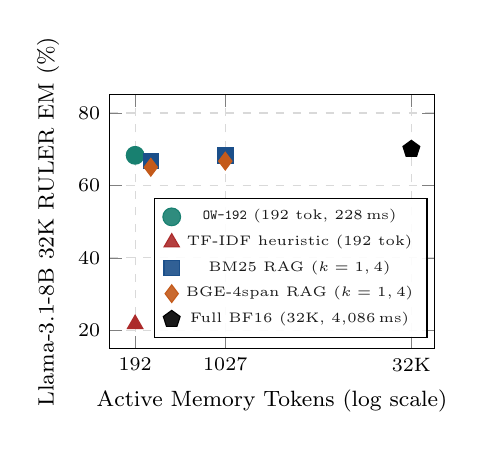
\begin{tikzpicture}
\begin{axis}[
    width=0.47\textwidth,
    height=4.8cm,
    xmode=log,
    xlabel={Active Memory Tokens (log scale)},
    ylabel={Llama-3.1-8B 32K RULER EM (\%)},
    ymin=15, ymax=85,
    xmin=120, xmax=50000,
    xtick={192,1027,32768},
    xticklabels={192,1027,32K},
    xlabel style={font=\footnotesize},
    ylabel style={font=\footnotesize},
    tick label style={font=\scriptsize},
    grid=major,
    grid style={dashed, gray!30},
    legend style={at={(0.98,0.04)}, anchor=south east, font=\tiny, fill=white, fill opacity=0.9}
]
\addplot[only marks, mark=*, mark size=3.2pt, color=tmlrteal] coordinates {(192, 68.3)};
\addlegendentry{\texttt{OW-192} ($192$ tok, $228\,\text{ms}$)}
\addplot[only marks, mark=triangle*, mark size=3.2pt, color=tmlrred] coordinates {(192, 21.7)};
\addlegendentry{TF-IDF heuristic ($192$ tok)}
\addplot[only marks, mark=square*, mark size=2.8pt, color=tmlrblue] coordinates {(257, 66.7) (1027, 68.3)};
\addlegendentry{BM25 RAG ($k=1,4$)}
\addplot[only marks, mark=diamond*, mark size=3.2pt, color=tmlrorange] coordinates {(257, 65.0) (1027, 66.7)};
\addlegendentry{BGE-4span RAG ($k=1,4$)}
\addplot[only marks, mark=pentagon*, mark size=3.2pt, color=black] coordinates {(32768, 70.0)};
\addlegendentry{Full BF16 ($32\text{K}$, $4{,}086\,\text{ms}$)}
\end{axis}
\end{tikzpicture}
\hfill
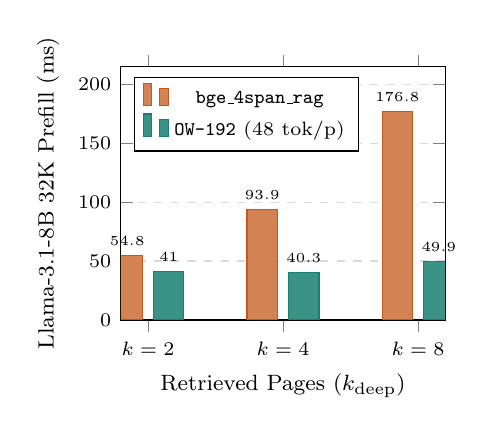
\begin{tikzpicture}
\begin{axis}[
    ybar=4pt,
    bar width=11pt,
    width=0.47\textwidth,
    height=4.8cm,
    ymin=0, ymax=215,
    ylabel={Llama-3.1-8B 32K Prefill (ms)},
    symbolic x coords={$k=2$, $k=4$, $k=8$},
    xtick=data,
    xlabel={Retrieved Pages ($k_{\text{deep}}$)},
    xlabel style={font=\footnotesize},
    ylabel style={font=\footnotesize},
    tick label style={font=\scriptsize},
    legend style={at={(0.04,0.96)}, anchor=north west, font=\scriptsize, fill=white},
    nodes near coords,
    nodes near coords style={font=\tiny, above},
    ymajorgrids=true,
    grid style={dashed, gray!30}
]
\addplot[fill=tmlrorange!75, draw=tmlrorange] coordinates {($k=2$, 54.8) ($k=4$, 93.9) ($k=8$, 176.8)};
\addplot[fill=tmlrteal!85, draw=tmlrteal] coordinates {($k=2$, 41.0) ($k=4$, 40.3) ($k=8$, 49.9)};
\legend{\texttt{bge\_4span\_rag}, \texttt{OW-192} ($48$ tok/p)}
\end{axis}
\end{tikzpicture}
\caption{\textbf{Left:} Accuracy vs.\ active memory tokens on $32\text{K}$ \texttt{RULER-style} retrieval (\texttt{Llama-3.1-8B-Instruct}; Section~\ref{sec:ruler}). \textbf{Right:} Unified $32\text{K}$ prefill latency scaling across $k_{\text{deep}} \in \{2,4,8\}$ on \texttt{Llama-3.1-8B-Instruct} ($2.33\times$ faster at $k=4$, $3.55\times$ at $k=8$, $-1.24\,\text{GiB}$ VRAM at $k=8$; Section~\ref{sec:twobank}). Full generation latency (including prefill, up to $32$ tokens with EOS) remains similar ($878$--$906\,\text{ms}$ vs.\ $890$--$984\,\text{ms}$).}
\label{fig:ruler_profile}
\end{figure}

\subsection{Cross-File Coding (65-File Repo, N=24)}
\label{sec:coding}
We evaluate multi-file Python API migration across $N=24$ synthetic $65$-file repositories with pathless retrieval queries (the generator prompt still receives the target caller file and task instruction, and \texttt{session\_notes} specifies \texttt{set \{kw\}=\{kw\_val\}}, explaining how \texttt{Llama-3.1-8B-Instruct} \texttt{bge\_4span\_rag\_k4} solves $3$ tasks without retrieving \texttt{core.py}). \texttt{chosen\_pages\_by\_caller} is verified $100\%$ identical ($0$ mismatches) between \texttt{OW-192} (\texttt{standalone\_discrete\_k4}) and \texttt{raw\_text\_same\_pages\_k4} on both backbones.

\begin{table}[t]
\centering
\caption{Cross-file Python API migration ($65$-file repos, $N=24$, unified single run per model). Among the displayed high-budget raw-text baselines, all comparisons with \texttt{OW-192} are non-significant at $N=24$ ($p \ge 0.109$; unadjusted Qwen wins over lower-$k$ JSON arms \texttt{bm25\_k4}/\texttt{k2} and \texttt{bge\_k2} are noted in text). The decisive coding finding is the $-79.2\pp$ collapse of \texttt{lslc\_full\_k4} ($p=3.81\times 10^{-6}$).}
\label{tab:coding}
\small
\resizebox{\textwidth}{!}{%
\begin{tabular}{@{}lcccc@{}}
\toprule
\textbf{System} & \textbf{Qwen3 \texttt{pass@1} [95\% CI]} & \textbf{Qwen3 Tok (\texttt{both/decoy})} & \textbf{Llama-8B \texttt{pass@1} [95\% CI]} & \textbf{Llama-8B Tok (\texttt{both/decoy})} \\
\midrule
\texttt{raw\_text\_same\_pages\_k4} & $\mathbf{24/24}$ ($100.0\%$) $[.862,1.00]$ & $356$ ($0.97 / 0.00$) & $22/24$ ($91.7\%$) $[.742,.977]$ & $337$ ($0.92 / 0.00$) \\
\texttt{OW-192} (\texttt{k4}) & $22/24$ ($91.7\%$) $[.742,.977]$ & $\mathbf{192}$ ($0.97 / 0.00$) & $21/24$ ($87.5\%$) $[.690,.957]$ & $\mathbf{192}$ ($0.92 / 0.00$) \\
\texttt{lslc\_exact\_only\_k4} & $20/24$ ($83.3\%$) $[.641,.933]$ & $192$ ($0.97 / 0.00$) & --- & --- \\
\texttt{bge\_4span\_rag\_k4} & $18/24$ ($75.0\%$) $[.551,.880]$ & $413$ ($0.61 / 0.04$) & $\mathbf{23/24}$ ($95.8\%$) $[.798,.993]$ & $412$ ($0.61 / 0.00$) \\
\texttt{bm25\_rag\_k8} & $16/24$ ($66.7\%$) $[.467,.820]$ & $1{,}038$ ($1.00 / 0.25$) & $\mathbf{23/24}$ ($95.8\%$) $[.798,.993]$ & $1{,}038$ ($1.00 / 0.00$) \\
\texttt{lslc\_full\_k4} ($+\vect{Z}_{\text{book}}$) & $1/24$ ($4.2\%$) $[.007,.203]$ & $312$ ($0.97 / 0.00$) & --- & --- \\
\bottomrule
\end{tabular}%
}
\end{table}

Table~\ref{tab:coding} shows that \texttt{raw\_text\_same\_pages\_k4} scores slightly higher than \texttt{OW-192} on both models ($24/24$ vs.\ $22/24$, $p=0.50$ on Qwen3; $22/24$ vs.\ $21/24$, $p=1.0$ on Llama-8B; in the full $11$-arm Qwen3 JSON, \texttt{OW-192} beats lower-$k$ raw baselines \texttt{bm25\_k4} $17$--$0$, $p=1.53\times 10^{-5}$, \texttt{bm25\_k2} $9$--$1$, $p=0.021$, and \texttt{bge\_k2} $10$--$1$, $p=0.012$ unadjusted). Thus, coding does \emph{not} show an accuracy advantage for discrete compression over matched raw text; it shows that $192$-token spans preserve $87.5\%$--$91.7\%$ \texttt{pass@1} at $1.85\times$ (Qwen3) / $1.76\times$ (Llama-8B) fewer tokens than matched raw text ($5.4\times$ fewer than \texttt{bm25\_rag\_k8}) while avoiding the latent-prefix collapse ($1/24$).

\subsection{Unified Systems Profile and Partitioned Two-Bank KV Reuse}
\label{sec:twobank}
Table~\ref{tab:profile_reuse} and Figure~\ref{fig:ruler_profile} (right) report the $32\text{K}$ unified systems profile alongside the partitioned Two-Bank KV-cache reuse sanity check across $P \in \{16, 64, 128\}$.

\begin{table}[t]
\centering
\caption{Unified $32\text{K}$ systems profile ($k_{\text{deep}} \in \{2,4,8\}$, generation up to $32$ tokens with EOS; \texttt{Full Gen} timer includes prefill) and partitioned Two-Bank KV reuse summary ($9$ configs per model: $P \in \{16,64,128\} \times \{\texttt{first\_p0}, \texttt{middle\_p1}, \texttt{last\_p\_end}\}$ for repeat Bank-2 edits $t_1 \rightarrow t_2$) on A100 40GB.}
\label{tab:profile_reuse}
\small
\setlength{\tabcolsep}{4.2pt}
\resizebox{\textwidth}{!}{%
\begin{tabular}{@{}lcccccc@{}}
\toprule
\textbf{32K Profile ($k_{\text{deep}}$)} & \textbf{BGE Prefill (ms)} & \textbf{\texttt{OW-192} Prefill (ms)} & \textbf{BGE Full Gen (ms)} & \textbf{\texttt{OW-192} Full Gen (ms)} & \textbf{BGE VRAM} & \textbf{\texttt{OW-192} VRAM} \\
\midrule
Qwen3 $k=2$ ($506$ vs.\ $96$ tok) & $45.1$ & $54.8$ ($0.82\times$) & $212.1$ & $150.1$ & $3{,}976\,\text{MiB}$ & $3{,}640\,\text{MiB}$ \\
Qwen3 $k=4$ ($1{,}013$ vs.\ $192$ tok) & $45.4$ & $44.2$ ($1.03\times$) & $235.9$ & $129.0$ & $4{,}382\,\text{MiB}$ & $3{,}717\,\text{MiB}$ \\
Qwen3 $k=8$ ($2{,}035$ vs.\ $384$ tok) & $65.4$ & $44.6$ ($1.47\times$) & $150.6$ & $129.5$ & $5{,}215\,\text{MiB}$ & $3{,}878\,\text{MiB}$ \\
\midrule
Llama-8B $k=2$ ($511$ vs.\ $96$ tok) & $54.8$ & $41.0$ ($1.34\times$) & $910.6$ & $881.5$ & $15{,}871\,\text{MiB}$ & $15{,}532\,\text{MiB}$ \\
Llama-8B $k=4$ ($1{,}022$ vs.\ $192$ tok) & $93.9$ & $\mathbf{40.3}$ ($\mathbf{2.33\times}$) & $889.8$ & $906.3$ & $16{,}244\,\text{MiB}$ & $15{,}610\,\text{MiB}$ \\
Llama-8B $k=8$ ($2{,}048$ vs.\ $384$ tok) & $176.8$ & $\mathbf{49.9}$ ($\mathbf{3.55\times}$) & $984.4$ & $877.9$ & $17{,}034\,\text{MiB}$ & $15{,}768\,\text{MiB}$ \\
\midrule
\textbf{Two-Bank KV Reuse ($t_1 \rightarrow t_2$)} & \textbf{Bank-1 Frac.} & \textbf{$\max|\Delta_{\text{KV}}|$} & \textbf{$\max|\Delta_{\text{logits}}|$} & \textbf{Full / Clone Reuse (ms)} & \textbf{Speed (Comp.)} & \textbf{Speed (Clone)} \\
\midrule
Qwen3 ($P \in \{16,64,128\}$, $232$ tok) & $65.1\%$ ($151$) & $0.0$ & $0.375$--$1.000$ & $43.7$--$44.7$ / $48.5$--$49.9$ & $0.93$--$0.95\times$ & $0.89$--$0.91\times$ \\
Llama-8B ($P \in \{16,64,128\}$, $230$ tok) & $66.5\%$ ($153$) & $0.0$ & $0.156$--$0.281$ & $39.8$--$41.1$ / $47.1$--$49.1$ & $0.87$--$0.91\times$ & $0.82$--$0.86\times$ \\
\bottomrule
\end{tabular}%
}
\end{table}

\paragraph{Two-Bank Prefix Invariance as a Sanity Check vs.\ Runtime Reality.}
Because causal attention depends only on preceding tokens, placing unedited pages deterministically in Bank~1 verifies \texttt{bank1\_embed\_max\_abs\_diff} $= 0.0$ and \texttt{bank1\_pkv\_max\_abs\_diff} $= 0.0$ over $65.1\%$--$66.5\%$ of prefix tokens across all $18$ tested configurations ($P \in \{16,64,128\}$). Three practical boundaries qualify this sanity check:
\begin{enumerate}
    \item \textbf{First-edit migration ($t_0 \rightarrow t_1$) vs.\ repeat edits ($t_1 \rightarrow t_2$):} The reuse harness applies Edit~\#1 first so the target page sits in Bank~2, then compares $t_1$ vs.\ $t_2$. On the \emph{first} mutation of a static page ($t_0 \rightarrow t_1$), moving \texttt{p0} from page order $[0,1,2,3]$ to $[1,2,3 \mid 0]$ invalidates the entire $4$-page memory slice (and moving \texttt{p1} retains only $1/4$ of the page slice, excluding prompt preamble tokens); invariance applies only to subsequent repeat edits to Bank~2.
    \item \textbf{BF16 logit drift and eager slowdown:} Chunked KV reuse vs.\ full re-prefill yields \texttt{final\_logits\_max\_abs\_diff} $\in [0.375, 1.000]$ on \texttt{Qwen3-1.7B} and $[0.156, 0.281]$ on \texttt{Llama-\allowbreak 3.1-8B-Instruct} (argmax token agreement was not logged), and eager HuggingFace \texttt{DynamicCache} reuse runs at $0.82\times$--$0.95\times$ the speed of full $230$-token re-prefill ($5\%$--$22\%$ slower). Whether zero-copy C++/PagedAttention servers~\citep{kwon2023vllm,zheng2024sglang} realize wall-clock gains at larger working sets remains untested.
    \item \textbf{Rerouting telemetry and encode/decode balance:} Across $72$ \texttt{Gate-2} transitions ($t_1 \rightarrow t_4$ repeating one budget query), exact Bank-1 page-sequence hit rate is $95.8\%$ (Qwen3, LCS $76.0\%$) and $100.0\%$ (Llama-8B, LCS $78.1\%$), dropping on $24$ high-churn Coding transitions to $0.0\%$ (Qwen3, LCS $15.6\%$) and $12.5\%$ (Llama-8B, LCS $17.7\%$). In the $32\text{K}$ ($k=4$) unified profile, \texttt{OW-192}'s encode ($164.0\,\text{ms}$ Llama, $161.0\,\text{ms}$ Qwen) exceeds BGE-RAG's ($110.7\,\text{ms}$ Llama, $117.6\,\text{ms}$ Qwen; note Table~\ref{tab:ruler}'s $148.3\,\text{ms}$ comes from the separate $32\text{K}$ RULER benchmark run), and warm full-generation time (which already includes prefill, max $32$ tokens with EOS) is comparable on Llama-8B ($906.3$ vs.\ $889.8\,\text{ms}$).
\end{enumerate}

% ===========================================================================
\section{Static Extractive Compression Boundary on \texttt{LongMemEval}}
\label{sec:lme}
% ===========================================================================

To probe how $48/256$-token extractive compression behaves on non-templated multi-session histories containing knowledge updates, we evaluate \texttt{OW-192} strictly in \textbf{static read-only extractive pruning + retrieval mode} (\textbf{$0$ calls to \texttt{apply\_edit}}, \texttt{EditGateHead}, or span-aligned overwrite) on all $N=72$ non-abstention \texttt{knowledge-update} items from \texttt{xiaowu0162/\allowbreak longmemeval-cleaned} (\texttt{longmemeval\_s\_cleaned.json}; LLM-simulated, human-curated chat histories~\citep{wu2025longmemeval}), alongside a stratified $N=30$ \texttt{Qwen3-1.7B} slice ($10$ \texttt{knowledge-update} items overlapping $N=72$, plus $10$ \texttt{single-session-user} and $10$ \texttt{multi-session}).

\paragraph{Packing Disclosure, Asymmetry, and Metric Definitions.}
Because full \texttt{LongMemEval} histories average $\sim 45$ sessions ($\sim 115\text{K}$ tokens), all runs use deterministic \texttt{gold\_prioritized\_64p} evidence-session packing, prioritizing \texttt{answer\_session\_ids} when truncating to \texttt{max\_pages} $=64$ ($\sim 7.7$ sessions retained; occasionally exceeding $64$ pages if gold sessions themselves are longer). This leaks evidence-session locations at packing time and saturates \texttt{session\_hit@k} $=1.000$ (at least one evidence session retrieved) across every arm. Moreover, because \texttt{bank.edited\_pages} is empty in static mode, \texttt{OW-192} orders its $4$--$6$ retrieved pages chronologically (\texttt{page\_id\_asc}), whereas RAG baselines order $k=2$ raw pages by descending relevance. We treat \textbf{\texttt{extracted\_em}} (first-clause normalized EM with leading-number matching for numeric golds) and \textbf{\texttt{token\_f1}} as primary metrics. We report two auxiliary diagnostics with explicit caveats:
\begin{itemize}
    \item \textbf{Lexical-coverage proxy (\texttt{pg $\rightarrow$ bk}):} When literal substring matching fails, the helper credits $1$ if all filtered gold content words appear anywhere across the combined retrieved pages or bank (regardless of word order or page boundaries). It is therefore an upper-bound lexical-coverage proxy rather than literal substring containment.
    \item \textbf{Exploratory \texttt{local\_value\_em}:} Included solely for completeness, as auditing per-episode outputs exposed three concrete failure modes of its unit-blind, order-blind numeric-set rule: crediting \texttt{"3 years."} for gold \texttt{"3 months"} (\texttt{Qwen3 d4}, \texttt{qid=2133c1b5}), crediting reversed update polarity (\emph{``led 5 initially, now 4''} vs.\ gold \emph{``4 initially, now 5''}; \texttt{Llama BM25}, \texttt{qid=031748ae}), and penalizing article variation (\texttt{"A music shop"} vs.\ \texttt{"The music shop"}, scoring $0$ despite \texttt{extracted\_em} $=1$, causing ValEM $<$ EM on \texttt{Llama d6}).
\end{itemize}

\begin{table}[t]
\centering
\caption{Static read-only QA on \texttt{LongMemEval} \texttt{knowledge-update} ($N=72$ non-abstention, \texttt{gold\_prioritized\_64p} packing, $0$ edit calls) and stratified $N=30$ (\texttt{Qwen3-1.7B}). Primary metrics are \texttt{Ext.\ EM} and \texttt{F1}; \texttt{Lex.\ Cov.} (\texttt{pg $\rightarrow$ bk}) is a bag-of-words lexical-coverage proxy, and \texttt{ValEM} is exploratory. Bold marks highest values per block (including ties).}
\label{tab:lme}
\small
\setlength{\tabcolsep}{4.2pt}
\resizebox{\textwidth}{!}{%
\begin{tabular}{@{}lcccccc@{}}
\toprule
\textbf{Benchmark \& Arm (Static Read-Only)} & \textbf{Ext.\ EM} & \textbf{Substr.} & \textbf{F1} & \textbf{Exp.\ ValEM} & \textbf{Lex.\ Cov.\ (\texttt{pg $\rightarrow$ bk})} & \textbf{Mem.\ Tok} \\
\midrule
\multicolumn{7}{@{}l@{}}{\textit{\texttt{Qwen/Qwen3-1.7B} --- \texttt{knowledge-update} ($N=72$)}} \\
\texttt{bm25\_rag\_k2} & $\mathbf{26.4\%}$ & $30.6\%$ & $36.0\%$ & $34.7\%$ & $59.7\%$ / --- & $510$ \\
\texttt{bge\_4span\_rag\_k2} & $\mathbf{26.4\%}$ & $\mathbf{33.3\%}$ & $\mathbf{38.3\%}$ & $\mathbf{38.9\%}$ & $58.3\%$ / --- & $507$ \\
\texttt{OW-192} static (\texttt{d4}, $48/256$) & $9.7\%$ & $9.7\%$ & $20.6\%$ & $13.9\%$ & $72.2\% \rightarrow 25.0\%$ & $192$ \\
\texttt{OW-192} static (\texttt{d6}, $48/256$) & $15.3\%$ & $15.3\%$ & $23.0\%$ & $18.1\%$ & $79.2\% \rightarrow 25.0\%$ & $288$ \\
\midrule
\multicolumn{7}{@{}l@{}}{\textit{\texttt{unsloth/Meta-Llama-3.1-8B-Instruct} BF16 --- \texttt{knowledge-update} ($N=72$)}} \\
\texttt{bm25\_rag\_k2} & $\mathbf{37.5\%}$ & $\mathbf{37.5\%}$ & $\mathbf{46.2\%}$ & $\mathbf{44.4\%}$ & $62.5\%$ / --- & $509$ \\
\texttt{bge\_4span\_rag\_k2} & $31.9\%$ & $31.9\%$ & $40.4\%$ & $37.5\%$ & $56.9\%$ / --- & $510$ \\
\texttt{OW-192} static (\texttt{d4}, $48/256$) & $23.6\%$ & $23.6\%$ & $29.0\%$ & $26.4\%$ & $68.1\% \rightarrow 33.3\%$ & $192$ \\
\texttt{OW-192} static (\texttt{d6}, $48/256$) & $31.9\%$ & $31.9\%$ & $36.1\%$ & $30.6\%$ & $79.2\% \rightarrow 38.9\%$ & $288$ \\
\midrule
\multicolumn{7}{@{}l@{}}{\textit{\texttt{Qwen/Qwen3-1.7B} --- Stratified Multi-Category ($N=30$; $10$ KU overlap with $N=72$)}} \\
\texttt{bge\_4span\_rag\_k2} / \texttt{bm25\_rag\_k2} & $\mathbf{33.3}/30.0\%$ & $\mathbf{33.3}/\mathbf{33.3\%}$ & $\mathbf{47.0}/40.5\%$ & $\mathbf{36.7}/\mathbf{36.7\%}$ & $56.7/60.0\%$ & $504/509$ \\
\texttt{OW-192} \texttt{d4} / \texttt{d6} / \texttt{lslc\_full} & $0.0/6.7/6.7\%$ & $0.0/10.0/6.7\%$ & $13.1/13.6/11.4\%$ & $3.3/13.3/10.0\%$ & $70/77/70\% \rightarrow 27/33/27\%$ & $192/288/330$ \\
\bottomrule
\end{tabular}%
}
\end{table}

\begin{figure}[t]
\centering
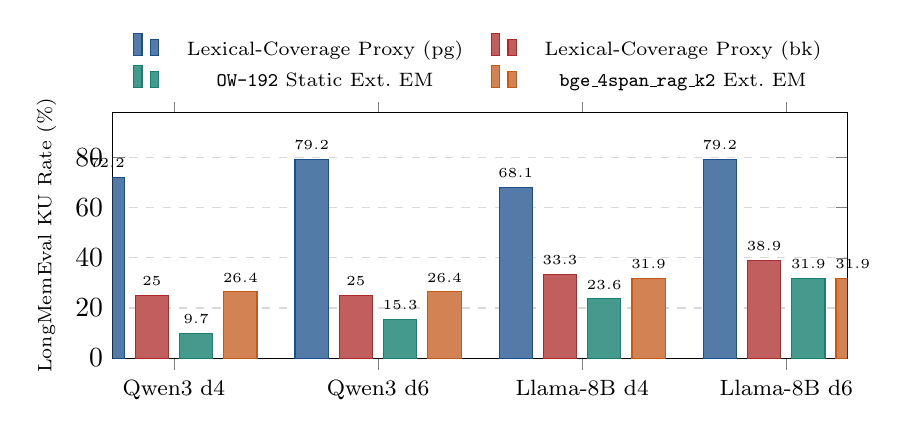
\begin{tikzpicture}
\begin{axis}[
    ybar=4pt,
    bar width=12pt,
    width=0.90\textwidth,
    height=4.7cm,
    ymin=0, ymax=98,
    ylabel={LongMemEval KU Rate (\%)},
    symbolic x coords={Qwen3 d4, Qwen3 d6, Llama-8B d4, Llama-8B d6},
    xtick=data,
    xticklabel style={font=\footnotesize},
    ylabel style={font=\scriptsize},
    legend style={at={(0.5,1.04)}, anchor=south, legend columns=2, column sep=8pt, font=\scriptsize, draw=none},
    nodes near coords,
    nodes near coords style={font=\tiny, above},
    ymajorgrids=true,
    grid style={dashed, gray!30}
]
\addplot[fill=tmlrblue!75, draw=tmlrblue] coordinates {(Qwen3 d4, 72.2) (Qwen3 d6, 79.2) (Llama-8B d4, 68.1) (Llama-8B d6, 79.2)};
\addplot[fill=tmlrred!75, draw=tmlrred] coordinates {(Qwen3 d4, 25.0) (Qwen3 d6, 25.0) (Llama-8B d4, 33.3) (Llama-8B d6, 38.9)};
\addplot[fill=tmlrteal!80, draw=tmlrteal] coordinates {(Qwen3 d4, 9.7) (Qwen3 d6, 15.3) (Llama-8B d4, 23.6) (Llama-8B d6, 31.9)};
\addplot[fill=tmlrorange!75, draw=tmlrorange] coordinates {(Qwen3 d4, 26.4) (Qwen3 d6, 26.4) (Llama-8B d4, 31.9) (Llama-8B d6, 31.9)};
\legend{Lexical-Coverage Proxy (pg), Lexical-Coverage Proxy (bk), \texttt{OW-192} Static Ext.\ EM, \texttt{bge\_4span\_rag\_k2} Ext.\ EM}
\end{axis}
\end{tikzpicture}
\caption{Static read-only compression boundary on \texttt{LongMemEval} \texttt{knowledge-update} ($N=72$, $0$ edit calls, \texttt{gold\_prioritized\_64p} packing). Dropping $81.25\%$ of tokens per page lowers the bag-of-words lexical-coverage proxy (\texttt{pg} $68\%$--$79\%$ $\rightarrow$ \texttt{bk} $25\%$--$39\%$) and trails raw-text RAG on \texttt{Qwen3-1.7B} primary \texttt{extracted\_em} ($9.7\%$--$15.3\%$ vs.\ $26.4\%$), while \texttt{Llama-3.1-8B-Instruct} \texttt{d6} ties \texttt{bge\_4span\_rag\_k2} in sample \texttt{extracted\_em} ($23/72 = 31.9\%$, $11$--$11$ discordant, paired CI $[-12.5, +12.5]\pp$).}
\label{fig:lme}
\end{figure}

Table~\ref{tab:lme} and Figure~\ref{fig:lme} delineate the boundary of $48/256$ static extractive pruning. On \texttt{Qwen3-1.7B} ($N=72$), \texttt{OW-192} static extraction trails \texttt{bge\_4span\_rag\_k2} on primary \texttt{extracted\_em} ($9.7\%$ \texttt{d4} and $15.3\%$ \texttt{d6} vs.\ $26.4\%$; raw $p=0.0227 / 0.1516$, Holm $p_{\text{H}}=0.136 / 0.606$ across $m=6$; exploratory \texttt{local\_value\_em} $p_{\text{H}}=0.0055 / 0.0407$), accompanied by a steep drop in the lexical-coverage proxy (\texttt{pg} $72.2\%$--$79.2\%$ $\rightarrow$ \texttt{bk} $25.0\%$; note that router, page count $k$, and page ordering also vary between RAG and static \texttt{OW-192}). On \texttt{Llama-3.1-8B-Instruct}, \texttt{OW-192} static \texttt{d6} ($288$ memory tok) attains the same sample \texttt{extracted\_em} as \texttt{bge\_4span\_rag\_k2} ($510$ memory tok) at $23/72$ ($31.9\%$; only $12$ items jointly correct, $11$--$11$ discordant, paired difference CI $[-12.5\pp, +12.5\pp]$, $p_{\text{H}}=1.0$---indistinguishable rather than proven equivalent), while trailing \texttt{bm25\_rag\_k2} ($37.5\%$ EM, $46.2\%$ F1, $p_{\text{H}}=1.0$). Because open-domain conversational facts lack consistent syntactic markers, dropping $81.25\%$ of tokens per page severely limits extractive recall on dialogue histories.

% ===========================================================================
\section{Limitations and Discussion}
\label{sec:limitations}
% ===========================================================================

We summarize seven explicit limitations bounding our findings:
\begin{enumerate}
    \item \textbf{Template scope, oracle write address, and prompt sensitivity:} \texttt{Gate-2} uses one synthetic template family ($6$ held-out eval values per mode; $35$ unique gold strings across $600$ \texttt{Qwen3-1.7B} episodes), single-seed evaluation on \texttt{Llama-3.1-8B-Instruct} ($N=200$), and shared oracle edit page addresses $p_i$ in Section~\ref{sec:gate2_factorial}. The edit gate classifies template acceptance phrasing rather than real-world factual authority. Our cluster bootstrap groups $( \texttt{mode}, \texttt{query\_type}, \texttt{gold} )$ rather than shared linguistic templates ($4$--$6$/type) or project names ($6$), and cluster-level sign-flip sensitivity weakens Holm-corrected inference on single-seed Llama ($p_{\text{sf,H}}=0.126$--$0.130$). Moreover, \texttt{Raw-App} did not include a prompt instruction favoring the latest update, so its gap could narrow under update-aware prompting.
    \item \textbf{No real-text online overwrite benchmark:} Section~\ref{sec:lme} evaluates \texttt{OW-192} strictly as a static read-only pruner ($0$ \texttt{apply\_edit} calls) with evidence-session packing. Validating gated in-place overwriting on open-domain streaming conversations remains open.
    \item \textbf{Short training budget of the latent prefix diagnostics:} Our latent diagnostics cover specific Perceiver-style input-space soft prefixes trained for $1{,}050$ post-adapter steps ($400+250+400$ atop an earlier released adapter checkpoint on \texttt{Qwen3-1.7B}) and $120$ steps (\texttt{Llama-3.1-8B-Instruct}, stopping at loss $3.52$). Longer pretraining or alternative injection architectures (e.g., mid-layer gated cross-attention avoiding $81\%$ token dropping) may behave differently.
    \item \textbf{Degenerate TF-IDF heuristic baseline:} On \texttt{Qwen3-1.7B}, \texttt{heuristic\_span16\_tfidf} drops to $0/60$ (including \texttt{s\_niah}) because digit-split BPE tokens have near-zero IDF; the large $+65\pp$ gap reflects this tokenizer pathology rather than comparison against a strong tuned extractive pruner.
    \item \textbf{Write latency, amortization, and storage overhead:} Mid-layer edit classification costs $\sim 40\,\text{ms/turn}$ ($172$--$186\,\text{ms}$ per $3$--$5$-turn episode), requiring $\ge 4$ queries/episode to break even on \texttt{Llama-3.1-8B-Instruct} and never breaking even on \texttt{Qwen3-1.7B}, while BGE indexing raises storage to $3{,}264$--$3{,}456\,\text{B/page}$ ($\sim 3\times$ bare UTF-8 text).
    \item \textbf{Two-Bank KV reuse is an invariance sanity check, not a runtime speedup:} Eager PyTorch \texttt{DynamicCache} reuse runs $5\%$--$22\%$ slower at $230$ tokens and introduces BF16 logit drift ($0.156$--$1.000$) without logged argmax token parity.
    \item \textbf{Provenance and checksum scope:} \texttt{max\_frozen\_param\_diff} $=0.0$ checks tensor-level FP32 sum and max-absolute checksums. Earlier runs recorded \texttt{git\_sha: unknown}, and the factorial/LongMemEval runs executed from a local source tarball layered over base commit \texttt{0e8f2d8}\ prior to final commit (Appendix~\ref{app:legacy}).
\end{enumerate}

% ===========================================================================
\section{Conclusion}
\label{sec:conclusion}
% ===========================================================================

Across two strictly frozen Transformer backbones (\texttt{Qwen3-1.7B} and \texttt{unsloth/\allowbreak Meta-\allowbreak Llama-\allowbreak 3.1-8B-Instruct}), our controlled study establishes two scoped empirical takeaways for editable compressed context memory. First, conditional on known edit addresses $p_i$, $4$ pages locked by \texttt{OW-192}'s post-edit router, and a $192$-token active memory budget on structured \texttt{Gate-2} templates, \textbf{span-aligned in-place overwrite (\texttt{OW-192})} consistently outperforms $31$-token rolling-tail append (\texttt{App-192}) by $+9.0\pp$ to $+15.0\pp$ across both page orders and backbones (replicated on $N=400$ fresh \texttt{Qwen3-1.7B} episodes at $+15.0\pp$, while noting cluster-level sign-flip sensitivity on single-seed Llama). However, \texttt{OW-192} does \emph{not} universally beat uncompressed in-place rewriting: on \texttt{Llama-3.1-8B-Instruct}, schema-aware \texttt{Raw-OW} ($1{,}030$ memory tokens) outperforms \texttt{OW-192} by $3.5\pp$--$6.5\pp$ on Norm-EM, $5.0\pp$--$8.5\pp$ on W2N-EM ($p_{\text{Holm}}=0.0116$ under \texttt{id\_asc}), and $99\%$ vs.\ $90\%$ ($91\%$ vs.\ $78\%$ \texttt{id\_asc}) on mutable queries. Second, our short-budget co-trained input-space continuous latent prefix displays a stark task-dependent interaction---producing $0/24$ masked-old verbatim readouts on both backbones, increasing continuation PPL, and collapsing \texttt{Qwen3-1.7B} Python coding ($1/24$ vs.\ $20/24$), while modestly assisting legacy suffix-overwrite \texttt{Gate-2} ($383/600$ vs.\ $351/600$). Finally, static read-only evaluation on \texttt{LongMemEval} \texttt{knowledge-update} ($N=72$) highlights the core bottleneck of $48/256$ extractive pruning on open-domain dialogue histories, motivating future in-model cross-attention memory architectures that retain full input coverage without dropping $81\%$ of tokens.

\subsubsection*{Broader Impact Statement}
This paper conducts a controlled diagnostic study of compressed editable memory for frozen language models using synthetic templates and publicly available benchmarks (\texttt{WikiText-2} and \texttt{LongMemEval}). Because the study does not train new frontier capabilities, collect private user data, or deploy autonomous agents, we anticipate no significant direct societal risks beyond standard considerations for frozen LLM inference. Documenting where short-budget latent prefixes fail verbatim updates and where aggressive extractive pruning loses conversational recall is intended to discourage unsafe over-reliance on lossy memory compression in high-stakes assistant settings.

% ===========================================================================

\bibliography{references}
\bibliographystyle{tmlr}

% ===========================================================================
\appendix
\section{Artifact Provenance, Checksums, and Legacy Seed Reference}
\label{app:legacy}
% ===========================================================================

All tables and figures reconcile to $17$ saved JSON artifacts under \texttt{evals/m2\_colab\_l4/} ($14$ evaluation files + $3$ training/diagnostic logs; offline cluster CIs for end-to-end Table~\ref{tab:gate2_e2e}, unrounded exact Holm $p$-values, cluster sign-flip checks, and legacy W2N rescoring are reproduced directly from saved per-episode rows by our CPU-only script \texttt{docs/reconcile\_paper\_metrics.py}) and $3$ locked \texttt{.safetensors} checkpoints (local unit test suite: $99/99$ tests passing):
\begin{itemize}
    \item \textbf{Path B \texttt{Qwen/Qwen3-1.7B} checkpoint:} \texttt{lslc\_pathb\_qwen3\_1.7b.safetensors} ($1{,}307{,}884\,\text{B}$, SHA-256 \texttt{\scriptsize\allowbreak 94cc5270b441a55a\allowbreak a87f8d99af8ca248\allowbreak d1f0ac465cf4aa48\allowbreak 52acb92f915613d0}); JSONs \texttt{v31\_qwen\_1..6*.json} (training + $5$ eval files, recorded \texttt{git\_sha: unknown}) and \texttt{v32\_tmlr\_qwen3\_1.7b.json} (source tarball layered over commit \texttt{0e8f2d8}).
    \item \textbf{Path B \texttt{unsloth/\allowbreak Meta-Llama-3.1-8B-Instruct} checkpoint:} \texttt{lslc\_pathb\_llama31\_8b.safetensors} ($2{,}381{,}052\,\text{B}$, SHA-256\\\texttt{\scriptsize 17c7918a6d9da31c\allowbreak 0640c94e902b8e4a\allowbreak 84d31264bbbd4597\allowbreak 97b250b5d06300fb}); JSONs \texttt{v31\_llama\_1..6*.json} and \texttt{v32\_tmlr\_llama31\_8b.json}.
    \item \textbf{Legacy \texttt{Qwen3-1.7B} universal checkpoint (\texttt{LSLC-Full} diagnostic baseline):} \texttt{lslc\_universal\_v2\_qwen3\_1.7b.safetensors} ($166{,}049{,}524\,\text{B}$, SHA-256 \texttt{\scriptsize 7048dfc167de9729\allowbreak a8507163b330a3c1\allowbreak ae46a5d8e517bdc7\allowbreak 2ffe2eb3323278e7}); JSONs \texttt{v3\_universal\_\allowbreak v2\_train.json} ($400$ steps, $67.05\,\text{s}$, warm-started from $250$-step \texttt{v3\_g2\_cond\_b.json} and $400$-step \texttt{v3\_s1\_r3\_frozen.json} atop an earlier adapter checkpoint: $1{,}050$ post-adapter steps total), \texttt{v3\_tb\_1\_edit\_masked\_old.json}, and legacy seeds $2026$--$2028$ \texttt{v3\_tb\_3\_gate2\_n200.json}.
    \item \textbf{Legacy \texttt{Gate-2} seeds $2026$--$2028$ (\texttt{v3\_tb\_3\_gate2\_n200.json}, $N=600$, prior to Span-Aligned Overwrite):} \texttt{bm25\_rag\_append\_errata} $51.83\%$ (W2N rescored via \texttt{canonicalize\_w2n\_answer}: $342/600 = 57.00\%$); \texttt{gated\_bm25\_rag} $47.83\%$ ($318/600 = 53.00\%$); legacy suffix-overwrite \texttt{standalone\_discrete} $58.83\%$ ($377/600 = 62.83\%$); \texttt{lslc\_full} $66.17\%$ ($422/600 = 70.33\%$).
\end{itemize}

\section{Gate-2 Prompt Template and Representative Episode}
\label{app:prompt}
All \texttt{Gate-2} arms prepend the exact $2$-shot formatting instructions below ahead of the query:
\begin{quote}\small\ttfamily
Format instructions: Reply with ONLY the concise exact value (matching unit format).\\
Example 1 -> Question: What is the approved budget for DemoA? Answer: 40M\\
Example 2 -> Question: What is the approved deployment state for DemoB? Answer: blue-green-prod
\end{quote}
In a representative \texttt{Gate-2} budget episode (\texttt{Qwen3-1.7B} factorial \texttt{episode\_idx=0}, \texttt{accepted\_override}), the $16$-page document places a static policy rule, the target project's initial \texttt{RECORD:} entry (page $p_i = 6$), and a neighbor project's record on three distinct pages amidst \texttt{WikiText-2} prose. Over $k=3$ edit turns directed to page $6$, accepted turns revise the project budget while rejected proposal turns decline alternative caps (often restating the previous value). Post-edit hybrid routing locks pages $[2, 6, 8, 9]$ across all $8$ arms; under \texttt{edited\_last}, pages are ordered $[2, 8, 9, 6]$ (placing mutated page $6$ last), and the target answer is \texttt{"85M"}.

\end{document}
